% \documentclass[a4paper,UKenglish,cleveref, autoref, thm-restate]{lipics-v2021}
% To anonymise:
\documentclass[a4paper,UKenglish,cleveref, autoref, thm-restate,anonymous]{lipics-v2021}

% \pdfoutput=1 %uncomment to ensure pdflatex processing (mandatatory e.g. to submit to arXiv)
\hideLIPIcs  %uncomment to remove references to LIPIcs series (logo, DOI, ...), e.g. when preparing a pre-final version to be uploaded to arXiv or another public repository

\bibliographystyle{plainurl}

\ifx\authoranonymous\relax
\newcommand{\GITHUBURL}{(anonymised)}
\newcommand{\COFFEEURL}{(anonymised)}
\else
\newcommand{\GITHUBURL}{\url{https://github.com/songlarknet/pipit}}
\newcommand{\COFFEEURL}{\url{https://youtu.be/6IybbQFPOl8}}
\fi

% is this package necessary?
\usepackage{mathtools}
\usepackage{mathpartir}

\usepackage{stmaryrd}

% checked box
\usepackage{wasysym}
\usepackage{underscore}

\usepackage{style/utils}
\usepackage{style/code}
\usepackage{style/proof}
\usepackage{style/keywords}
\usepackage{style/judgements}


\title{Pipit on the Post: Proving Pre- and Post-conditions of Reactive Systems}


\author{Amos Robinson}{Australian National University, Canberra, Australia}{amos.robinson@anu.edu.au}{https://orcid.org/0009-0004-4837-4981}{}

\author{Alex Potanin}{Australian National University, Canberra, Australia}{alex.potanin@anu.edu.au}{https://orcid.org/0000-0002-4242-2725}{}

\authorrunning{A. Robinson and A. Potanin}
\Copyright{Amos Robinson and Alex Potanin}
% \ccsdesc[300]{Computer systems organization~Embedded software}
\ccsdesc[500]{Computer systems organization~Real-time languages}
\ccsdesc[500]{Theory of computation~Program verification}
% \ccsdesc[100]{Theory of computation~Modal and temporal logics}
\ccsdesc[500]{Software and its engineering~Specialized application languages}
\keywords{Lustre, streaming, reactive, verification}

% \category{}

\begin{document}

\maketitle

\begin{abstract}
  Reactive languages such as Lustre and Scade are used to implement safety-critical control systems; proving such programs correct and having the proved properties apply to the compiled code is therefore equally critical.
  We introduce Pipit, a small reactive language embedded in \fstar{}, designed for verifying control systems and executing them in real-time.
  Pipit includes a verified translation to transition systems; by reusing \fstar{}'s existing proof automation, certain safety properties can be automatically proved by k-induction on the transition system.
  Pipit can also generate executable code in a subset of \fstar{} which is suitable for compilation and real-time execution on embedded devices.
  The executable code is deterministic and total and preserves the semantics of the original program.
\end{abstract}


% enable @verbatim@ syntax
\makeatactive


%!TEX root = ../Main.tex
\section{Introduction}

Data flow fusion~\cite{lippmeier2013flow} is a technique to compile a specific class of data flow programs into single, efficient imperative loops. This process of ``compilation'' is equivalent to performing array fusion on a combinator based functional array program, as per related work on stream fusion~\cite{coutts2007streamfusion} and delayed arrays~\cite{keller2010repa}. The key benefits of data flow fusion over this prior work are: 1) it fuses programs that use branching data flows where a produced array is consumed by several consumers, and 2) complete fusion into a single loop is guaranteed for all programs that operate on the same size input data, and contain no fusion-preventing dependencies between operators.

Fusion-preventing dependencies express the fact that some operators simply must wait for others to complete before they can produce their own output. For example, in the following:
\begin{code}
  normalize :: Array Int -> Array Int
  normalize xs = let sum = fold (+) 0 xs
                 in  map (/ sum) xs
\end{code}

If we wish to divide every element of an array by the sum of all elements, then it seems we are forever destined to compute the result using at least two loops: one to determine the sum, and one to divide the elements. The evaluation of @fold@ demands all elements of its source array, and we cannot produce any elements of the result array until we know the value of @sum@. 

However, many programs \emph{do} contain opportunities for fusion, if we only knew which opportunities to take. The following example offers \emph{several} unique, but mutually exclusive approaches to fusion. Figure~\ref{f:normalize2-cluterings} on the next page shows some of the possibilities.
\begin{code}
 normalize2 :: Array Int -> Array Int
 normalize2 xs
  = let sum1 = fold   (+)  0   xs
        gts  = filter (> 0)    xs
        sum2 = fold   (+)  0   gts
        ys1  = map    (/ sum1) xs
        ys2  = map    (/ sum2) xs
    in (ys1, ys2)
\end{code}

In Figure~\ref{f:normalize2-cluterings}, the dotted lines show possible clusterings of operators. Stream fusion implicitly choses the solution on the left as its compilation process cannot fuse a produced array into multiple consumers. The best existing ILP approach will chose the solution on the right as it cannot cluster operators that consume arrays of different lengths. Our system choses the solution in the middle, which is also optimal for this example. 

% NOTE: This set of bullets needs to fit on the first page, without spilling to the second.
Our contributions are as follows:
\begin{itemize}
\item   
We extend prior work by Megiddo~\cite{megiddo1998optimal} and Darte~\cite{darte2002contraction}, with support for length changing operators. Length changing operators can be clustered with the operators that generate their source arrays, and compiled naturally with data-flow fusion (\S\ref{s:ILP}).

\item
We present a simplification to constraint generation that is also applicable to some existing integer linear programming formulations such as Megiddo's,
where constraints between two nodes need not be generated if there exists a fusion-preventing path between the two (\S\ref{s:OptimisedConstraints}).

\item
Our constraint system also encodes a total ordering on the cost of clusterings, expressed using weights on the integer linear program. For example, we encode that memory traffic is more expensive than loop overheads, so given a choice between the two, the memory traffic will be reduced (\S\ref{s:ObjectiveFunction}).

\item
We present benchmarks of our algorithm applied to several common programming patterns, and to several pathological examples.
Our algorithm is complete and yields good results in practice, though if array sizes are unknown, an optimal solution is uncomputable in general. \TODO{ref}
\end{itemize}

The reduction of the clustering problem to integer linear programming was previously described by~\cite{megiddo1998optimal}, though they do not consider length changing operators.


% We must also decide which clustering is the `best' or most optimal. One obvious criterion for this is the minimum number of loops, but there may even be multiple clusterings with the minimum number of loops. In this case, the number of required manifest arrays must also be taken into account. 

% As real programs contain tens or hundreds of individual operators, performing an exhaustive search for an optimal clustering is not feasible, and greedy algorithms tend to produce poor solutions. 


%!TEX root = ../Main.tex

\section{Pipit for time-triggered networks}
\label{s:motivation}

% Pure streaming languages like Lustre lie in an uneasy space somewhere between pure functions and imperative programs.
% Like pure functions, pure streaming languages are equational and support reasoning by unfolding and rewriting.
% Like imperative programs, they describe how state evolves over time.
% Additionally, Lustre programs tend to be composed of many nested recursive loops.
% When verifying both pure and imperative programs, recursion or loops generally require explicit loop invariants.
% Requiring an explicit invariant for each recursive stream quickly becomes unwieldy for Lustre programs.

To introduce Pipit, we consider a driver with a static schedule of \emph{triggers}, or actions to be performed at a particular time; this driver is a simplification of the time-triggered CAN bus specification \cite{fuehrer2001time} which we will discuss further in \autoref{s:evaluation}.
% In this system, time is partitioned into a sequence of \emph{cycles}; at the start of each new cycle, the time is reset to zero.
% Triggers also have a cycle offset and a repeat factor, which together determine the cycles in which the trigger is active.

\subsection{Deferring and proving properties}

The schedule of our time-triggered driver is determined by a constant array of triggers, sorted by their associated time-mark; the driver maintains an index that refers to the current trigger.
At each instant in time, the driver checks if the current trigger has expired or is inactive, and if so, it increments the index.
We first implement a streaming function \emph{count_when} to maintain the index; the function takes a constant natural number \emph{max} and a stream of booleans \emph{inc}.
At each time step, \emph{count_when} checks whether the current increment flag is true; if so, it increments the previous counter, saturating at the maximum; otherwise, it leaves the previous counter as-is.

\begin{tabbing}
  @MM@\= @MM@ \= \kill
  @let@ count_when ($\textit{max}$: $\NN$) ($\textit{inc}$: stream $\BB$): stream $\NN$ = \\
    \> $@rec@~\rawbind{\textit{count}}{}$ \\
    \> \> $\xcheckP{\PSUnknown}{(0 \le \textit{count} \le \textit{max})}$; \\
    \> \> @let@ $\textit{count'}$ @=@ $(0~@fby@~\textit{count}) + (@if@~\textit{inc}~@then@~1~@else@~0)$ @in@ \\
    \> \> @if @ $\textit{count'} \ge \textit{max}$ @then@ $\textit{max}$  @else@ $\textit{count'}$
\end{tabbing}

The implementation of \emph{count_when} first defines a recursive stream, \emph{count}, which states an invariant about the count before defining the incremented stream \emph{count'}.
Inside \emph{count'}, the syntax $0~@fby@~\textit{count}$ is read as ``the initial value of zero \emph{followed by} the previous count''.

The syntax $\xcheckP{\PSUnknown}{(0 \le \textit{count} \le \textit{max})}$ asserts that the count is within the range $[0, \textit{max}]$.
The subscript $\PSUnknown$ on the check is the \emph{property status}, which in this case denotes that the assertion has been stated, but it is not yet known whether it holds.
A property status of $\PSValid$, on the other hand, denotes that a property has been proved to hold.
These property statuses are used to defer checking properties until enough is known about the environment, and to avoid rechecking properties that have already been proven.
In practice, the user does not explicitly specify property statuses in the source language.
The stated property $(0 \le \textit{count} \le \textit{max})$ is a stream of booleans which must always be true.
% \footnote{We limit our scope to safety properties: in real-time systems, liveness properties tend to be easily restated as bounded liveness properties, which are a form of safety property \cite{manna2012temporal}}
Non-streaming operations such as $\le$ are implicitly lifted to streaming operations, and non-streaming values such as $0$ and $\textit{max}$ are implicitly lifted to constant streams.

We defer the proof of the property here because, at the point of stating the property inside the @rec@ combinator, we don't yet have a concrete definition for the count variable.
In this case, we could have instead deferred the \emph{statement} of the property by introducing a let-binding for the recursive count and putting the @check@ outside of the @rec@ combinator.
However, it is not always possible to defer property statements: for example, when calling other streaming functions that have their own preconditions, it may not be possible to move the function call outside of its enclosing @rec@.
% In such cases, it is necessary to defer the proof of the precondition.

Pipit is an embedded domain-specific language.
The program above is really syntactic sugar for an \fstar{} program that takes a natural number and constructs a Pipit core expression with a free boolean variable.
We will discuss the details of the core language in \autoref{s:core}, but for now we will show the source program with some minor embedding details omitted.

To actually prove the property above, we use the meta-language \fstar{}'s tactics to translate the program into a transition system and prove the property inductively on the system.
Finally, we \emph{bless} the expression, which marks the properties as valid ($[\PSUnknown := \PSValid]$).
Blessing is an intensional operation: it traverses the expression and updates the internal metadata, but it does not affect the runtime semantics.

\begin{tabbing}
  @MM@\= @MM@ \= \kill
  @let@ $\mbox{count_when}_{\PSValid}$ ($\textit{max}$: $\NN$): stream $\BB$ $\to$ stream $\NN$ = \\
    \> @let@ $\textit{system} = \mbox{System.translate}_1 (\mbox{count_when}~\textit{max})$ @in@ \\
    \> @assert@ (System.inductive_check $\textit{system}$) @by@ (pipit_simplify ()); \\
    \> $@bless@_1$ $(\mbox{count_when}~\textit{max})$
\end{tabbing}

The subscript 1 in the translation to transition system and blessing operations refers to the fact that the stream function has one stream parameter.
The \emph{pipit_simplify} tactic in the assertion performs normalisation-by-evaluation to simplify away the translation to a first-order transition system; \fstar{}'s proof-by-SMT can then solve the inductive check directly.
% This proof does require some boilerplate; in the future we hope to minimise this.

Callers of \emph{count_when} can now use the validated variant without needing to re-prove the count-range property.
In a dedicated model-checker such as Kind2 \cite{champion2016kind2} or Lesar \cite{raymond2008synchronous}, this kind of bookkeeping would all be performed under-the-hood.
By embedding Pipit in a general-purpose theorem prover, we move some of the bookkeeping burden onto the user; however, we have increased confidence that the compiled code matches the verified code and, as we shall see, we also have access to a rich specification language.
% As an embedded language, we also benefit from writing our programs in a rich metalanguage.

\subsection{The time-triggered system matrix}

The schedule of the time-triggered network is abstractly described by a \emph{system matrix}, consisting of rows of \emph{basic cycles}, columns of \emph{transmission columns}, and cells of optional messages.
Each basic cycle is identified by its cycle index and each transmission column has an associated time-mark.

\autoref{f:tt-systemmatrix-ok} (left) shows an example system matrix with cycles @C0@ and @C1@ and transmission columns at time-marks 0, 1 and 2.
For this example, we assume that one message can be sent per clock cycle. % , though in practice a message could take on the order of ten microseconds
To execute this system matrix, we synchronise the local time to zero at the start of basic cycle @C0@.
After a basic cycle completes, the nodes on the network synchronise before execution continues to the next basic cycle.

\autoref{f:tt-systemmatrix-ok} (right) shows the corresponding configuration for the triggers array.
The enabled set denotes the basic cycles for which a trigger is active.

The system has strict timing requirements, which restrict how triggers can be defined.
In this example, each trigger has a unique time; in general, trigger times can overlap, but they need to be enabled on distinct cycles.
Additionally, the schedule must allow sufficient time for the driver to skip over any disabled triggers.
Concretely, we could postpone trigger 1 to send message @B@ at time-mark 2 instead.
However, we could not bring forward trigger 2 to send message @C@ at time-mark 1: the driver can only process one trigger per time-mark, and it takes two steps to reach trigger 2 from the start of the array.

\begin{figure}
  \begin{minipage}{0.38\textwidth}
\begin{tabular}{r|ccc}
   & TM0 & TM1 & TM2 \\
  \hline
  C0 & MSG A & MSG B & - \\
  C1 & MSG A & - & MSG C
\end{tabular}
\end{minipage}
\begin{minipage}{0.6\textwidth}
\small
\begin{verbatim}
  0: { time_mark = 0; enabled = {C0,C1}; msg = A; }
  1: { time_mark = 1; enabled = {C0};    msg = B; }
  2: { time_mark = 2; enabled = {C1};    msg = C; }
\end{verbatim}
\end{minipage}
  
\caption{Left: system matrix; right: corresponding triggers array configuration}
\label{f:tt-systemmatrix-ok}
\end{figure}

% The time-marks are strict deadlines on the order of microseconds, which prohibits the driver from looping through the whole array at each time step to find the next active trigger.
% Instead, the driver maintains an index that refers to the current trigger; at each instant in time, the driver checks if the current trigger has expired or is inactive, and if so, it increments the index.
% Multiple triggers can have the same time-mark, as long as they are active in different cycles; triggers that are active on the same cycle must have a sufficiently wide gap in their time-marks to allow the driver time to iterate through the inactive triggers between them and reach the next active trigger before it starts.
% The implementation itself is simple, but formalising exactly what constitutes a ``sufficiently wide gap'' and proving that the schedule is never late requires care.

We impose three main restrictions on the triggers array: it must be sorted; there must be an adequate time-gap between any two triggers that are enabled on the same cycle index; and each trigger's time-mark must be greater-than-or-equal to its index.

With these restrictions in place, we prove a lemma \emph{lemma_can_reach_next}, which states that for all valid cycle indices and trigger indices, if the current trigger is enabled in the current cycle and there is another enabled trigger scheduled to occur somewhere in the array after the current one, then there is an adequate time-gap to allow the driver to skip over any disabled triggers in-between.
These properties are fairly straightforward in a theorem prover, but would be difficult to state in a model-checker with a limited specification language.

% \begin{figure}
%   \begin{minipage}{0.38\textwidth}
% \begin{tabular}{r|c}
%    & TM0 \\
%   \hline
%   C0 & MSG A \\
%   C1 & MSG B
% \end{tabular}
% \end{minipage}
% \begin{minipage}{0.6\textwidth}
%   \small
%   \begin{verbatim}
%     { time_mark =  0; enabled = {C0}; msg = A; }
%     { time_mark =  0; enabled = {C1}; msg = B; }
%   \end{verbatim}
%   \end{minipage}
  
% \caption{Invalid trigger configuration}
% \label{f:tt-systemmatrix-bad}
% \end{figure}

\subsection{Instantiating lemmas and defining contracts}
\label{s:motivation:contract}

% The trigger-fetch logic requires such a combination of automatic and manual proofs.
We can now implement the trigger-fetch logic, which maintains the index that refers to the next-scheduled trigger.
The trigger-fetch logic uses the \emph{count_when} streaming function to define the index; the increment flag given to count_when will increment the index if the previous index has expired or is inactive in the current cycle.
We simplify our presentation here and only consider a single cycle in isolation: the real system presented in \autoref{s:evaluation} has some extra complexity such as resetting the index, incrementing the cycle index at the start of a new cycle, and using machine integers.

\begin{tabbing}
  @MM@\= @MM@ \= @let index@ \= \kill
  @let@ trigger_fetch ($\textit{cycle}$: $\NN$) ($\textit{time}$: stream $\NN$): stream $\NN$ = \\
    \> $@rec @ \textit{index}.$ \\
    \> \> $@let @ \textit{inc} = \text{false} @ fby @ ((\text{time_mark}~\textit{index}) \le \textit{time} ~\vee~ \neg (\text{enabled}~\textit{index}~\textit{cycle})) @ in@$\\
    \> \> $@let @ \textit{index} = \mbox{count_when}_{\PSValid}~\text{trigger_count}~\textit{inc} @ in@$ \\
    \> \> $\text{pose}_1~(\text{lemma_can_reach_next}~\textit{cycle})~\textit{index}$; \\
    \> \> $\xcheckP{\PSUnknown}{(\text{can_reach_next_active}~\textit{cycle}~\textit{time}~\textit{index})}$; \\
    \> \> $\textit{index}$\\
\end{tabbing}

The \emph{trigger_fetch} function takes a static cycle index and the stream denoting the current time.
The increment flag and the index are mutually dependent --- the increment flag depends on the previous value of the index, while the index depends on the current value of the increment flag --- so we introduce a recursive stream for the index.
We allow the index to go one past the end of the array to denote that there are no more triggers.

We use the $\textit{pose}_1$ helper function to lift the \emph{lemma_can_reach_next} lemma to a streaming context and instantiate it; the subscript 1 refers to the lemma taking one streaming argument (the index).
% The lemma requires a non-streaming cycle and a non-streaming index; we apply it to the static cycle and the combinator lifts the application to the streaming index.
% The $\textit{pose}$ function is a helper function implemented using the @check@ and @bless@ functions from earlier.
% The property we state here is that if the trigger at the current index is active, then there is a sufficient time gap to be able to reach the next active trigger after the current index.
We then state an invariant as a deferred property.
Informally, the invariant states that, either the current active trigger is not late, or the next active trigger after the current index is in the future and we can reach it in time.

With the explicitly instantiated lemma, we can prove the streaming invariant by straightforward induction on the transition system.
To help make proofs of the rest of the system more compositional, we also abstract over the details of the trigger-fetch mechanism by introducing a rely-guarantee contract for \emph{trigger_fetch}.
The contract we state is that if the environment always ensures that the time doesn't skip --- that is, we are called once per microsecond --- then we guarantee that we never encounter a late trigger.

\begin{tabbing}
  @MM@\= @MM@ \= @MMMMMMMMMMMMM@ \= \kill
  @let@ $\text{trigger_fetch}_{\PSValid}$ ($\textit{cycle}$: $\NN$): $\stream \NN \to \stream \NN$ = \\
  \> @let@ $\textit{contract} = \text{Contract.contract_of_stream}_1$ \{ \\
  \> \> @rely@ = $(\lambda \textit{time}.~ \text{time_no_skips}~\textit{time} )$ \\
  \> \> @guar@ = $(\lambda \textit{time index}.~ (\text{index_valid}~\textit{index} \wedge \text{enabled}~\textit{index}~\textit{cycle})$ \\
  \> \> \> $\implies (\text{time_mark}~\textit{index}) \ge \textit{now})$ \\
  \> \> @body@ = $(\lambda \textit{time}.~ \text{trigger_fetch}~\textit{cycle}~\textit{time} )$ \\
  \> \} @in@ \\
  \> @assert@ $(\text{Contract.inductive_check}~\textit{contract})$ @by@ (pipit_simplify ()); \\
  \> $\text{Contract.stream_of_contract}_1~\textit{contract}$
\end{tabbing}

In the implementation of the validated variant of \emph{trigger_fetch}, we first construct the contract from streaming functions.
The $\text{Contract.contract_of_stream}_1$ combinator describes a contract with one input (the time stream), and takes stream transformers for each of the rely, guarantee and body.
The combinator transforms the surface syntax into core expressions.
The assertion $(\text{Contract.inductive_check}~\textit{contract})$ then translates the expressions into a transition system, and checks that if the rely always holds then the guarantee always holds, and that the as-yet-unchecked subproperties hold.
Finally, $\text{Contract.stream_of_contract}_1$ blesses the core expression and converts it back to a stream transformer, so it can be easily used by other parts of the program.

When this function is used in other parts of the program, the caller must ensure that the environment satisfies the rely clause.
In the core language, this is tracked by another deferred property status attached to the contract; we will discuss this further in \autoref{s:core}.
% Deferring the proof of the rely clause is crucial for function calls where satisfying the precondition at a particular point in time somehow depends on the value of the output at a previous step.
% These kinds of self-dependencies and mutual-dependencies are fairly common in Lustre-style programs: for example, \emph{trigger_fetch}'s invocation of \emph{count_when}, whose input $\textit{inc}$ depends on the previous output $\textit{index}$.


%!TEX root = ../Main.tex

% \pagebreak
\section{Pipit core language}
\label{s:core}

%!TEX root = ../Main.tex
\begin{figure}
  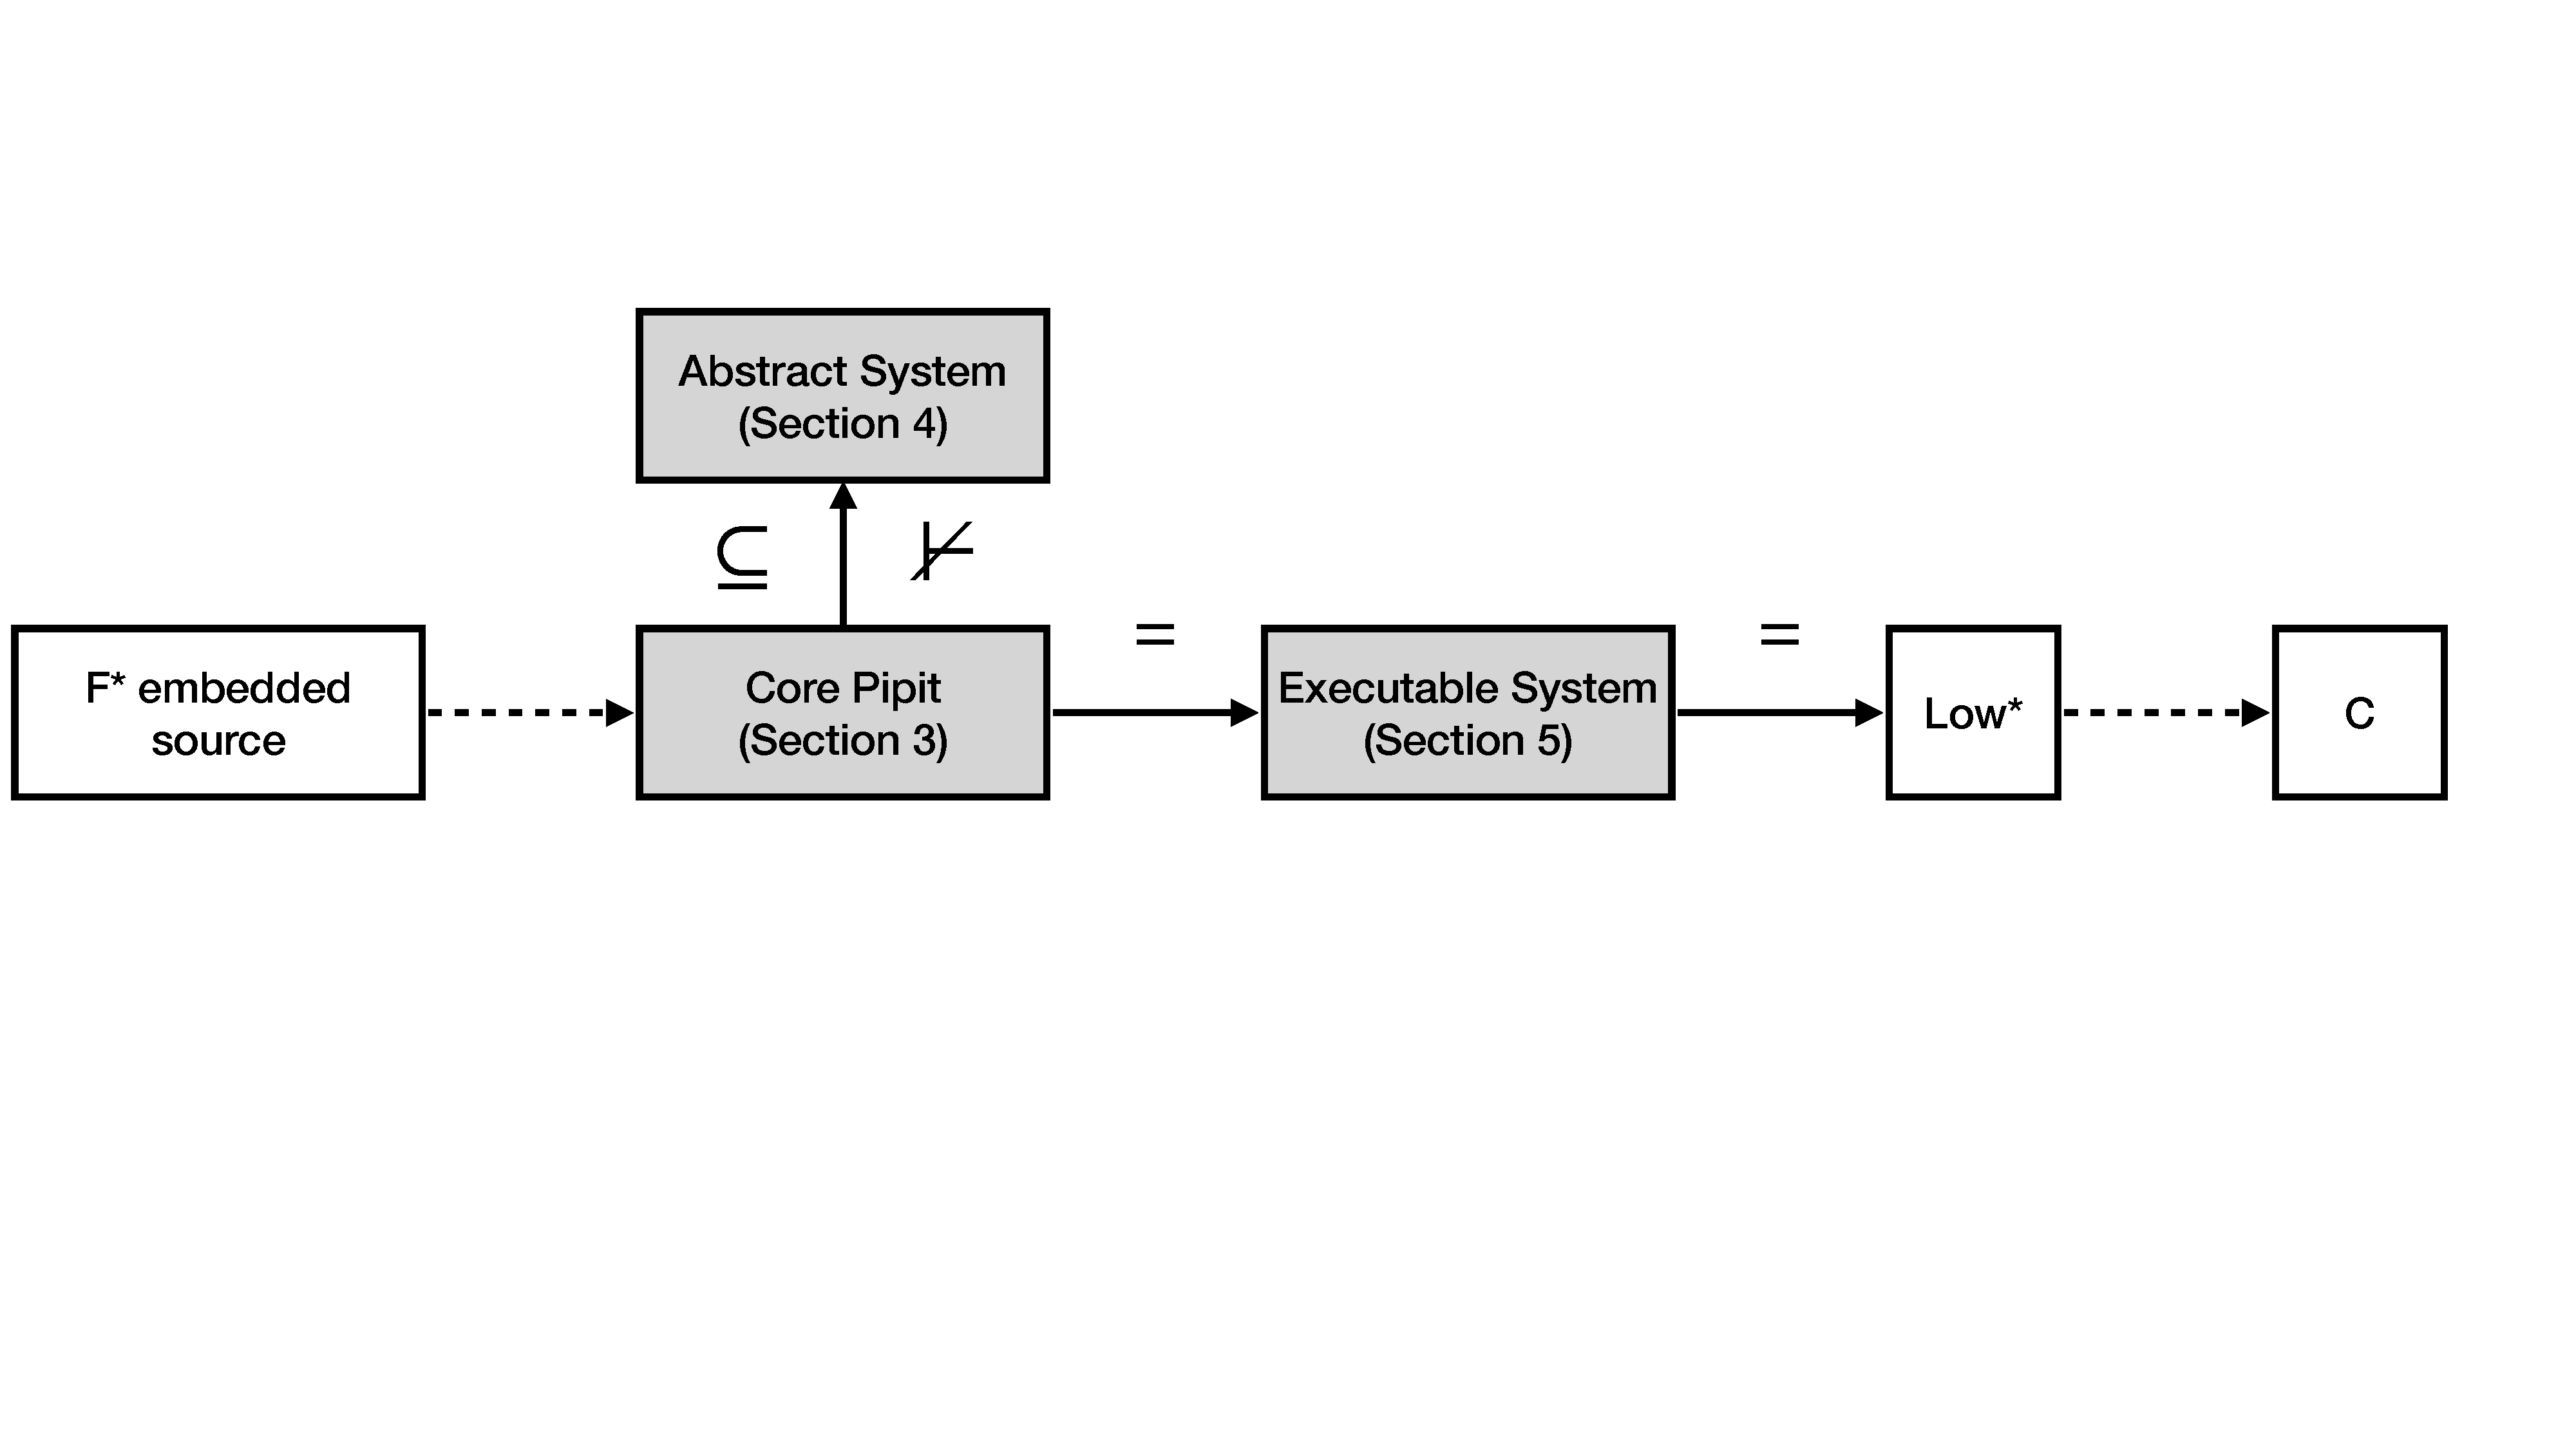
\includegraphics[width=\textwidth]{figures/core-structure.pdf}
\caption{Architecture of Pipit. The gray boxes and solid arrows are defined in this paper. The white boxes and dashed arrows are trusted components. The labels next to the arrows denote properties of the translation. The refinement label ($\subseteq$) indicates a verified abstraction relation; the negated entailment ($\not\vdash$) indicates that the entailment relation --- contracts and checked properties proven on abstract system apply to the checked semantics --- is not yet verified; the equivalence ($=$) denotes a verified equivalence relation.}
\label{f:core:structure}
\end{figure}


We now introduce the core Pipit language.
Note that this form differs slightly from the surface syntax presented earlier in \autoref{s:motivation}, which used the syntax of the metalanguage \fstar{}, as well as including proofs in \fstar{} itself.


\autoref{f:core:structure} shows the high-level architecture of Pipit.
On the left-hand-side, the surface syntax embedded in \fstar{} is shown; this includes some Pipit-specific syntactic sugar.
The translation from the surface syntax to the core language is trusted.
There are two targets from the core language: abstract transition systems for verification, and executable transition systems for extraction to C.
The translation to abstract systems is verified to be an abstraction according to the dynamic semantics (\autoref{s:core:dynamic}).
The translation to abstract systems also generates proof obligations, which are verified to correspond to the proof obligations on the original program.
% One property that still remains to be proven is that the proof obligations on the abstract transition system entail the original proof obligations (\autoref{s:transition}); this pending proof is denoted as negated entailment in the figure ($\not\vdash$).
The translation to executable transition systems is proven to be semantics-preserving, as is the subsequent translation to \lowstar{}.
The translation from \lowstar{} to C is external to this paper and forms part of our trusted computing base.


\autoref{f:core-grammar} defines the grammar of Pipit.
The expression form $e$ includes standard syntax for values ($v$), variables ($x$) and primitive applications ($p(\ov{e})$).
Most of the expression forms were introduced informally in \autoref{s:motivation} and correspond to the clock-free expressions of Lustre~\cite{caspi1995functional}.

%!TEX root = ../Main.tex

\begin{figure}
  \[
  \begin{array}{lrlr}
    e, e' & := & v ~|~ x ~|~ p(\ov{e}) & \mbox{(values, variables and operations)} \\
          & | & \xfby{v}{e} ~|~ \xrec{x}{e[x]} & \mbox{(followed-by (delay) and recursive streams)} \\ % & | & \xthen{e}{e'} \\
          & | & \xlet{x}{e}{e'[x]} & \mbox{(let-expressions)}\\
          & | & \xcheckP{\PStatus}{e_{\text{prop}}} & \mbox{(checked properties)} \\
          & | & \xcontractP{\PStatus}{\erely}{\eimpl}{x\!.~\eguar} & \mbox{(rely-guarantee contracts)} \\
          % & | & \xcheck{e} \\
    \\
    v & := & n \in \mathbb{N} ~|~ b \in \mathbb{B} ~|~ r \in \mathbb{R} ~|~ \hdots  & \mbox{(values)} \\
    p & := & (+) ~|~ (-) ~|~ (\times) ~|~ @if-then-else@ ~|~ \hdots & \mbox{(primitives)} \\
    \\
    \PStatus & := & \PSValid ~|~ \PSUnknown & \mbox{(property statuses: valid or unknown)}\\
    \\
    \sigma & := & \sgl{\ov{x \mapsto v}} & \mbox{(heaps)} \\
    \Sigma & := & \sigma ~|~ \Sigma;\sigma & \mbox{(streaming history environments)} \\
    %   \\
    \tau, \tau' & := & \mathbb{N} ~|~ \mathbb{B} ~|~ \tau \times \tau ~|~ \hdots & \mbox{(value types)} \\
    \Gamma & := & \cdot ~|~ x : \tau, \Gamma & \mbox{(type environments)}  \\
    \end{array}
  \]
  \caption{Pipit core language grammar, which contains expressions $e$, values $v$, primitive operations $p$, and property statuses $\PStatus$.}
  \label{f:core-grammar}
\end{figure}

The expression syntax for delayed streams ($\xfby{v}{e}$) denotes the previous value of the stream $e$, with an initial value of $v$ when there is no previous value.
% Streams can also be composed together using the \emph{then} notation ($\xthen{e}{e'}$) which denotes that the value of stream $e$ is used for the first step, followed by the values from stream $e'$ for subsequent steps.

Recursive streams are defined using the fixpoint operator ($\xrec{x}{e[x]}$); the syntax $e[x]$ means that the variable $x$ can occur in $e$.
% To ensure that streams are productive,
As in Lustre, recursive streams can only refer to their previous values and must be \emph{guarded} by a delay: the stream $(\xrec{x}{\xfby{0}{(x + 1)}})$ is well-defined and counts from zero up, but stream $(\xrec{x}{x + 1})$ is invalid and has no computational interpretation.
This form of recursion differs slightly from standard Lustre, which uses a set of mutually-recursive bindings.
% We use this form to define a substitution-based operational semantics that is syntax-directed, as opposed to the mutually-recursive form in \cite{caspi1995functional} which is not syntax-directed.
% Our semantics has a simpler proof of determinism; we believe it has simplified other necessary proofs too and will perform further evaluation.
Although we cannot express mutually-recursive bindings in the core syntax here, we can express them as a notation on the surface syntax by combining the bindings together into a record or tuple.

Checked properties and contracts are annotated with their property status $\PStatus$, which can either be valid ($\PSValid$) or unknown ($\PSUnknown$).
For checked properies $\xcheckP{\PStatus}{e}$, the property status denotes whether the property has been proved to be valid.

Contracts $\xcontractP{\PStatus}{\erely}{\ebody}{\rawbind{x}\eguar[x]}$ involve two verification conditions.
Firstly, when a contract is \emph{defined}, the definer must prove that the body satisfies the contract: roughly, if $\erely$ is always true, then $\eguar[x := \ebody]$ is always true.
Secondly, when a contract is \emph{instantiated}, the caller must prove that the environment satisfies the precondition: that is, $\erely$ is always true.
Conceptually, then, a contract could have two property statuses: one for the definition and one for the instantiation.
However, in practice, it is not useful to defer the proof of a contract definition --- one could achieve a similar effect by replacing the contract with its implementation.
For this reason, we only annotate contracts with one property status, which denotes whether the instantiation has been proved to satisfy the precondition.

For example, the core expression $\sumrec$ computes the sum of values from a stream of integers $i$ by defining a recursive stream $\sumvar$, which is delayed and given an initial value of zero.
If we were to use this sum in a context that required a strictly positive integer, we could give it a contract that states that if the input stream is always positive, then the resulting sum is also positive:
$$
\sumcontract
$$
To be considered a valid program, we must prove that the contract definition itself holds, as with our earlier contract (\autoref{s:motivation:contract}).
The unknown property status here allows us to defer the caller's proof that the input stream is always positive until the contract is used.


The remaining grammatical constructs of \autoref{f:core-grammar} describe streams, value environments, types and type environments.
Streams $V$ are represented as a sequence of values; streaming history environments $\Sigma$ are streams of heaps.
Types $\tau$ and type environments $\Gamma$ are standard.
For the presentation of the formal grammar here, we consider only a fixed set of values and primitives; in practice, the implementation is parameterised by a primitive table which we extend with immutable array operations for the TTCAN driver logic in \autoref{s:evaluation}.

\begin{figure}
  \[
    \boxed{\typing{\Gamma}{e}{\tau}}
    \quad
    \boxed{\mtyping{}{v}{\tau}}
  \]

  \[
    \ruleIN{
      \mtyping{}{v}{\tau}
    }{
      \typing{\Gamma}{v}{\tau}
    }{TValue}
    \quad
    \ruleAx{\typing{\Gamma}{x}{\Gamma(v)}}{TVar}
  \]

  \[
    \ruleIN{
      \typing{\Gamma}{e}{\tau \to \tau'}
      \qquad
      \typing{\Gamma}{e'}{\tau}
    }{\typing{\Gamma}{e~e'}{\tau'}}{TApp}
  \]

  \[
    \ruleIN{
      \typing{\Gamma}{v}{\tau}
      \qquad
      \typing{\Gamma}{e'}{\tau}
    }{
      \typing{\Gamma}{\xfby{v}{e'}}{\tau}
    }{TFby}
  \]

  \[
    \ruleIN{
      \typing{\Gamma}{e}{\tau}
      \qquad
      \typing{\Gamma}{e'}{\tau}
    }{\typing{\Gamma}{\xthen{e}{e'}}{\tau}}{TThen}
  \]

  \[
    \ruleIN{
      \typing{x : \tau, \Gamma}{e}{\tau}
    }{
      \typing{\Gamma}{\xrec{x}{e[x]}}{\tau}
    }{TRec}
  \]

  \[
    \ruleIN{
      \typing{\Gamma}{e}{\tau}
      \qquad
      \typing{x : \tau, \Gamma}{e'}{\tau'}
    }{
      \typing{\Gamma}{\xlet{x}{e}{e'[x]}}{\tau'}
    }{TLet}
  \]

  \[
    \ruleIN{
      \typing{\Gamma}{e}{\mathbb{B}}
    }{
      \typing{\Gamma}{\xcheck{e}}{\tt{unit}}
    }{TCheck}
  \]

  \caption{Typing rules for Pipit defined in terms of two judgment forms: $\typing{\Gamma}{e}{\tau}$ denotes that expression $e$ describes a \emph{stream} of values of type $\tau$; and $\mtyping{}{v}{\tau}$, which denotes that closed meta-value $v$ has type $\tau$ and is not defined here.}\label{f:core-typing}
\end{figure}

We define the typing judgments for Pipit in \autoref{f:core-typing}.
Most of the typing rules are standard for an unclocked Lustre.
The typing judgment $\typing{\Gamma}{e}{\tau}$ denotes that, in an environment of streams $\Gamma$, expression $e$ denotes a stream of type $\tau$.
This core typing judgment differs from the surface syntax used in \autoref{s:motivation}, which used an explicit stream type; for the core language, we instead assume that everything is a stream.

For values, we use an auxiliary definition $\mtypingval{v}{\tau}$ to denote that value $v$ has type $\tau$.
Likewise, for primitives we use $\mtypingprim{p}{(\tau_1 \times \cdots \hdots \times \tau_n) \to \tau'}$ to denote that primitive $p$ takes arguments of type $\tau_i$ and returns a result of type $\tau'$.
Primitives are pure, non-streaming functions.

Rules \textsc{TValue}, \textsc{TVar}, \textsc{TPrim} and \textsc{TLet} are standard.

Rule \textsc{TFby} states that expression $\xfby{v}{e}$ requires both $v$ and $e$ to have equal types; the result is the same type.

Rule \textsc{TRec} states that a recursive stream $\xrec{x}{e}$ has the recursive stream bound inside $e$.
The recursion must also be guarded, in that any recursive references to $x$ are delayed, but this requirement is performed as a separate syntactic check described in \autoref{s:core:causality}.

Rule \textsc{TCheck} states that statically checking a property $\xcheckP{\PStatus}{e}$ requires a boolean property $e$ and returns unit.

Finally, rule \textsc{TContract} applies for a contract $\xcontractP{\PStatus}{\erely}{\ebody}{\rawbind{x}\eguar[x]}$ with a body expression of some type $\tau$.
The overall expression has result type $\tau$.
Both rely and guarantee clauses must be boolean expressions.
Additionally, the guarantee clause can refer to the result value as $x$.

\subsection{Dynamic semantics}
\label{s:core:dynamic}
\begin{figure}
  \[ \boxed{\bigstep{\Sigma}{e}{v}} \]

  \[
    \ruleAx{\bigstep{\Sigma}{v}{v}}{Value}
    \quad
    \ruleAx{\bigstep{\Sigma_\bot; \sigma}{x}{\sigma(v)}}{Var}
  \]

  \[
    \ruleIN{
      \bigstep{\Sigma}{e}{(\mlamX)}
      \qquad
      \bigstep{\Sigma}{e'}{v'}
    }{\bigstep{\Sigma}{e~e'}{(\mlamX)~v'}}{App-Meta}
  \]

  % \[
  %   \ruleIN{\bigstep{\Sigma}{e}{v}}{\bigstep{\Sigma; \sigma}{\xpre{e}}{v}}{Pre}
  % \]

  \[
    \ruleAx{\bigstep{\sigma}{\xfby{v}{e'}}{v}}{$\mbox{Fby}_1$}
    \quad
    \ruleIN{\bigstep{\Sigma}{e'}{v'}}{\bigstep{\Sigma; \sigma}{\xfby{v}{e'}}{v'}}{$\mbox{Fby}_S$}
  \]

  \[
    \ruleIN{\bigstep{\sigma}{e}{v}}{\bigstep{\sigma}{\xthen{e}{e'}}{v}}{$\xthenarrow_1$}
    \quad
    \ruleIN{\bigstep{\Sigma}{e'}{v'}}{\bigstep{\Sigma; \sigma}{\xthen{e}{e'}}{v'}}{$\xthenarrow_S$}
  \]

  \[
    \ruleIN{
      \bigstep{\Sigma}{e[x := \xrec{x}{e}]}{v}
    }{
      \bigstep{\Sigma}{\xrec{x}{e[x]}}{v}
    }{Rec}
  \]

  \[
    \ruleIN{
      \bigstep{\Sigma}{e'[x := e]}{v}
    }{
      \bigstep{\Sigma}{\xlet{x}{e}{e'[x]}}{v}
    }{Let}
  \]

  \[
    \ruleIN{
      \bigstep{\Sigma}{e}{\top}
    }{
      \bigstep{\Sigma}{\xcheck{e}}{()}
    }{Check}
  \]

  \caption{Bigstep operational semantics for Pipit defined in terms of the judgment form $\bigstep{\Sigma}{e}{v}$; this judgment form denotes that evaluating expression $e$ under streaming history $\Sigma$ results in value $v$.}\label{f:core-bigstep}
\end{figure}

The dynamic semantics of Pipit are defined in \autoref{f:core-bigstep}.
We present our semantics in a big-step form.
This differs somewhat from traditional \emph{reactive} semantics of Lustre~\cite{caspi1995functional}.
Our big-step semantics emphasises the equational nature of Pipit, as it is substitution-based and syntax-directed, while the reactive semantics emphasises the finite-state streaming execution of the system.
We use transition systems for reasoning about the finite-state execution (\autoref{s:transition}), which is fairly standard~\cite{brun2023equation,champion2016kind2,raymond2008synchronous}.
Previous work on the {\sc W-calculus}~\cite{gallego2021w} for linear digital-signal-processing filters makes a similar distinction and provides a non-streaming semantics for reasoning about programs and a streaming semantics for executing programs.


The judgment form $\bigstep{\Sigma}{e}{v}$ denotes that expression $e$ evaluates to value $v$ under streaming history $\Sigma$.
The streaming history is a stream of heaps; in practice, we only evaluate expressions with a non-empty streaming history.

At a high level, evaluation proceeds by unfolding the recursive streams until a concrete value is determined.
For example, to evaluate the earlier sum example with input stream $i = [1; 2]$, we start with the judgment:
$$
\bigstep{\sumionetwo}{\sumrec}{v}
$$

First, we unfold the recursive stream to get $(\xfby{0}{\sumrec}) + i$.
To evaluate variables, we look for the variable in the current, or most recent, heap:
$$
\ruleIN{
}{
  \bigstep{\sumionetwo}{i}{2}
}{Var}
$$

For delays, we discard the current heap and continue evaluation with the history prefix:
$$
\ruleIN{
  \bigstep{\sgl{i \mapsto 1}}{\sumrec}{1}
}{
  \bigstep{\sumionetwo}{\xfby{0}{\sumrec}}{1}
}{$\mbox{Fby}_S$}
$$

Returning to \autoref{f:core-bigstep}, rule {\sc Value} states that evaluating a value results in the value itself.
Rule {\sc Var} states that to evalute a variable $x$ under some non-empty stream history $\Sigma; \sigma$, where $\sigma$ is the most recent heap, we look up the variable in $\sigma$.
Rule {\sc Prim} states that to evaluate a primitive $p$ applied to many arguments $e_1$ to $e_n$, we evaluate each argument separately; we then apply the primitive with prim-sem metafunction.
Rule {\sc Let} is standard.

For delay expressions $\xfby{v}{e}$, we have two cases depending on whether there is a previous value or not.
When there is no previous value -- the streaming history consists of just the current heap -- rule $\textsc{Fby}_1$ evaluates to the default value $v$.
Otherwise, rule $\textsc{Fby}_S$ applies.
In this case, the rule evaluates the previous value of $e$ by discarding the most recent entry from the streaming history.

Rule {\sc Rec} evaluates a recursive stream $\xrec{x}{e}$ by unfolding the recursion one step.
For causal expressions (\autoref{s:core:causality}), where each recursive occurrence of $x$ is guarded by a followed-by, this unfolding eventually terminates as each followed-by shortens the history.

Rule {\sc Check} states that check expressions always evaluate to unit.
We do not perform a dynamic check that the property is true here; checking the truth of properties is dealt with in the checked semantics (\autoref{s:core:checked}).

Rule {\sc Contract} states that contracts evaluate by just evaluating their body.
Like with checks, we do not perform a dynamic check that the precondition and postcondition hold.
From an abstraction perspective, it would be valid to return an arbitrary value that satisfies the contract.
However, such an abstraction would make evaluation non-deterministic and, for contracts with unsatisfiable postconditions, non-total.
The deterministic and total nature of evaluation is key to our proofs and metatheory.

We also define two auxiliary judgment forms: $\bigsteps{\Sigma}{e}{V}$ and $\bigstepalways{\Sigma}{e}$.

Judgment form $\bigsteps{\Sigma}{e}{V}$ denotes that, under history $\Sigma$, expression $e$ evaluates to the \emph{stream} $V$.
This judgment performs iterated application of single-value evaluation.

Judgment form $\bigstepalways{\Sigma}{e}$ denotes that a boolean expression $e$ evaluates to the stream of trues under history $\Sigma$.
Informally, it can be read as ``$e$ is always true in history $\Sigma$''.

\subsection{Checked semantics}
\label{s:core:checked}

In addition to the big-step semantics above, we also define a judgment form for checking that the properties and contracts of a program hold for a particular streaming history.
We call these the \emph{checked} semantics.
Unlike an axiomatic semantics, the checked semantics operate on a concrete set of input streams.

The checked semantics have the judgment form $\semcheck{\Sigma}{\PStatus}{e}$, which denotes that under streaming history $\Sigma$, the properties of $e$ with status $\PStatus$ hold.
The property status dictates which properties should be checked and which should be ignored.

To show that an expression $e$'s unknown properties hold, we prove that for all streaming histories $\Sigma$, assuming the valid properties hold ($\semcheck{\Sigma}{\PSValid}{e}$), then the unknown properties ($\semcheck{\Sigma}{\PSUnknown}{e}$) hold.
The assumption here means that we do not have to re-check properties after proving them once.

Contracts involve two proofs: one for the definition and one for the instantiation.
To prove that a contract definition $\xcontractP{\PStatus}{\erely}{\ebody}{\rawbind{x}\eguar[x]}$ is valid, we show that for all streaming histories $\Sigma$, assuming the rely is always true under the history ($\bigstepalways{\Sigma}{\erely}$), and assuming that the body evaluates to some stream $V$ ($\bigsteps{\Sigma}{\ebody}{V}$), then the guarantee always holds ($\bigstepalways{\Sigma[x \mapsto V]}{\eguar}$).
Additionally, we can also assume that the valid properties in all three components hold, and we must also show that the unknown properties are valid.
The fact that the checked semantics refers to a particular $\Sigma$ is significant here: it allows the proof of contract validity to only consider streaming histories where the rely actually holds.

% and the unknown properties in the body and guarantee both hold ($\semcheck{\Sigma}{\PSUnknown}{\ebody} \wedge \semcheck{\Sigma}{\PSUnknown}{\eguar[x := \ebody]}$).
% and assuming that the valid properties in the rely, body and guarantee hold ($\semcheck{\Sigma}{\PSValid}{\erely} \wedge \semcheck{\Sigma}{\PSValid}{\ebody} \wedge \semcheck{\Sigma}{\PSValid}{\eguar[x := \ebody]}$)

For example, recall our earlier sum contract, which stated that the sum of strictly positive integers is itself positive:
$$
@let@~\text{sum}~i = \sumcontract
$$
To check the contract definition on a concrete input $i = [1; 2]$, we first evaluate the body:
$$
\bigsteps{\sumionetwo}{\sumrec}{[1; 3]}
$$
We then check that, assuming all inputs are positive, then all results are positive:
$$
\bigstepalways{\sumionetwo}{i > 0} \implies
\bigstepalways{\sgl{i \mapsto 1, \sumvar \mapsto 1}; \sgl{i \mapsto 2, \sumvar \mapsto 3}}{sum > 0}
$$

To prove that the contract definition is valid for all inputs, we perform a similar proof for arbitrary input streams ($\forall \Sigma$).
We assume that the rely is true \emph{at all points} in the stream, and must show that the guarantee is true \emph{at all points}.
Consider if we had instead used the input stream $i = [-10; 1]$; here, the rely is false at the first step, but is instantaneously true at the second step.
In this case, the sum is $-10$ at the first step, and $-9$ at the second step.
At both steps the output is negative and the guarantee is false, even though the rely becomes true at the second step.
This behaviour is a key difference between streaming contracts and imperative pre-post contracts, which consider their preconditions in isolation.

Contract instantiations often involve feedback loops, where the input to a contract depends, directly or indirectly, on previous output values of the contract itself.
For example, we can compute the Fibonacci sequence by instantiating the sum contract with its output fed back to it\footnote{The program shown here does not strictly fit within the core grammar, which does not support named functions; in the implementation we use the \fstar{} meta-language's top-level definitions for such definitions.}:
$$
  % @rec@~\fibvar.\, \sumcontractX{\PSUnknown}{(\xfby{1}{\fibvar})}
  @rec@~\fibvar.\, \text{sum}~(\xfby{1}{\fibvar})
$$

To prove this instantiation valid, we need to show that the input $(\xfby{1}{\fibvar})$ is positive.
To do this, we perform induction on the input streams, allowing us to assume that the rely was previously true.
We then use the contract to show that, if the rely was true at the previous step, then the guarantee was true at the previous step -- which implies that the previous result is positive.
We describe the mechanisms of this proof in \autoref{s:transition}.

% To prove that a contract \emph{instantiation} (a call-site) is valid, we show that, under the calling environment, the rely clause is always true.
% Crucially, the proof can also use the fact that, if the rely is always true, then the guarantee is always true.
% This sort of feedback is necessary for proving properties of mutually-dependent calls.
This circular dependency is well-founded as our causality check ensures that recursive streams are guarded by delays (\autoref{s:core:causality}).
For example, the non-causal program $@rec@~\textit{nope}.\, \text{sum}~(-\textit{nope})$ depends instantaneously on itself.
The rely requires that the negated result is positive; the guarantee ensures that the result is positive.
However, there is no positive number whose negation is also positive, therefore the rely cannot imply the guarantee.
This potential issue is resolved by outlawing such non-causal programs.

%!TEX root = ../Main.tex

\begin{figure}
  \begin{mathpar}
    \boxed{\semcheck{\Sigma}{\PStatus}{e}}
  \end{mathpar}

  \begin{mathpar}
    \ruleAx{\semcheck{\Sigma}{\PStatus}{v}}{ChkValue}
    \quad
    \ruleAx{\semcheck{\Sigma}{\PStatus}{x}}{ChkVar}

    \ruleIN{
      \semcheck{\Sigma}{\PStatus}{e_1} \quad \hdots \quad
      \semcheck{\Sigma}{\PStatus}{e_n}
    }{\semcheck{\Sigma}{\PStatus}{p(\ov{e})}}{ChkPrim}


    \ruleIN{\semcheck{\Sigma}{\PStatus}{e'}}{\semcheck{\Sigma}{\PStatus}{\xfby{v}{e'}}}{ChkFby}

    \ruleIN{
      \bigsteps{\Sigma}{\xrec{x}{e}}{V}
      \and
      \semcheck{\Sigma[x \mapsto V]}{\PStatus}{e}
    }{
      \semcheck{\Sigma}{\PStatus}{\xrec{x}{e[x]}}
    }{ChkRec}

    \ruleIN{
      \semcheck{\Sigma}{\PStatus}{e}
      \and
      \bigsteps{\Sigma}{e}{V}
      \and
      \semcheck{\Sigma[x \mapsto V]}{\PStatus}{e'}
    }{
      \semcheck{\Sigma}{\PStatus}{\xlet{x}{e}{e'[x]}}
    }{ChkLet}

    \ruleIN{
      (\PStatus = \PStatus' \implies \bigstepalways{\Sigma}{e})
      \and
      \semcheck{\Sigma}{\PStatus}{e}
    }{
      \semcheck{\Sigma}{\PStatus}{\xcheckP{\PStatus'}{e}}
    }{ChkCheck}

    % \ruleIN{
    %   \PStatus \neq \PStatus'
    % }{
    %   \semcheck{\Sigma}{\PStatus}{\xcheckP{\PStatus'}{e}}
    % }{ChkNoCheck}

    \inferrule{
      \bigsteps{\Sigma}{\ebody}{V}
      \\\\
      (\PStatus = \PStatus' \implies \bigstepalways{\Sigma}{\erely})
      \\\\
      (\PStatus = \PSValid \implies \bigstepalways{\Sigma}{\erely} \implies \bigstepalways{\Sigma[x \mapsto V]}{\eguar})
      \\\\
      \semcheck{\Sigma}{\PStatus}{\erely}
      \\\\
      (\bigstepalways{\Sigma}{\erely} \implies \semcheck{\Sigma}{\PStatus}{\ebody} ~\wedge~ \semcheck{\Sigma[x \mapsto V]}{\PStatus}{\eguar})
    }{
      \semcheck{\Sigma}{\PStatus}{\xcontractP{\PStatus'}{\erely}{\ebody}{\rawbind{x}{\eguar[x]}}}
    }(\textsc{ChkContract})

    % \ruleIN{
    %   \PStatus \neq \PStatus'
    %   \and
    %   (\bigstepalways{\Sigma}{\erely}
    %    \implies \bigstepalways{\Sigma}{\eguar[x := \ebody]})
    % }{
    %   \semcheck{\Sigma}{\PStatus}{\xcontractP{\PStatus'}{\erely}{\ebody}{\rawbind{x}{\eguar[x]}}}
    % }{ChkNoContract}
  \end{mathpar}

  \caption{Checked semantics for Pipit; the judgment form $\semcheck{\Sigma}{\PStatus}{e}$ denotes that evaluating expression $e$ under streaming history $\Sigma$ satisfies the checks and rely-guarantee contract requirements that are labelled with property status $\PStatus$.}\label{f:core-check}
\end{figure}


The checked semantics of Pipit is defined in \autoref{f:core-check}.
The checked semantics descends into the expression and checks the properties and contracts as they are encountered.
For binding forms such as let-expressions and recursive-expressions, the semantics evaluates the corresponding expression and extends the streaming history with the bound variable.

Rules {\sc ChkValue} and {\sc ChkVar} state that values and variables are always valid.

Rule {\sc ChkPrim} checks a primitive application by descending into the subexpressions.
Similarly, rule {\sc ChkFby} descends into followed-by expressions.

Rule {\sc ChkRec} checks a recursive-expression $\xrec{x}{e}$ by evaluating the overall expression to a stream of values $V$.
The rule then extends the streaming environment $\Sigma$ with $x$ bound to the values from $V$; this extended environment is used to descend into the recursive expression.

Rule {\sc ChkLet} checks a let-expression $\xlet{x}{e}{e'}$ descends into both sub-expressions.
To check the body $e'$, the rule first evaluates $e$ and extends the streaming environment.

Finally, the heavy lifting is performed by rules {\sc ChkCheck} and {\sc ChkContract}.

Rule {\sc ChkCheck} applies when checking property status $\PStatus$ of an expression $\xcheckP{\PStatus'}{e}$.
If the check-expression has the same status as what we are checking ($\PStatus = \PStatus'$), then we perform the actual check by evaluating the expression $e$ and requiring it to evaluate to a stream of trues.
Otherwise, we do not need to evaluate the check-expression.
In both cases, we descend into the expression and check its subexpressions, as they may have nested properties.
Such nested properties are unlikely to be written directly by the user, but might occur after program transformations such as inlining.

Rule {\sc ChkContract} applies when checking property status $\PStatus$ of a contract with expression $\xcontractP{\PStatus'}{\erely}{\ebody}{\rawbind{x}\eguar[x]}$.
First, we evaluate the body to a stream $V$; these values are used to check that the body satisfies guarantee.
Although we only include one property status on the contract, conceptually there are two distinct properties: one for the caller ($\PStatus'$) and one for the definition itself (assumed to be $\PSValid$).
To check the caller property when $\PStatus = \PStatus'$, we evaluate the rely $\erely$ and require it to hold.
To check the definition property when $\PStatus = \PSValid$, we assume that the rely holds, and check that the body satisfies the guarantee.
We also descend into the subexpressions to check them; when checking the body and guarantee, we can assume that the rely holds.
% This rule must deal with the two different roles of a contract at once; in the next section, we will separate the two roles.

We do not generally verify programs directly using the checked semantics.
Instead, the checked semantics is intended as a specification describing what it means to be a valid program.
To verify concrete programs, we generally translate to an abstract transition system and construct the proofs there (\autoref{s:transition}).
% The semantics for contracts is fairly subtle, but we believe it is simpler than the translation to transition systems.
% Having a relatively simple high-level semantics of checks and contracts leaves room for future optimisations in translation to abstract transition systems.
% Additionally, existing contract support in Kind2~\cite{champion2016kind2} has rather ad-hoc restrictions, such as disallowing calling other contracts inside contract relies and guarantees. Our semantics handles this case without any special treatment.

\subsubsection{Blessing expressions and contracts}
\label{s:core:blessing}

Blessing is a meta-operation that replaces the property statuses in an expression so that all checks and contracts are marked as valid ($\PSValid$).
Blessing an expression requires a proof that the checked semantics hold for all input streams:

$$
\ruleIN{
  \forall \Sigma.~
  \semcheck{\Sigma}{\PSValid}{e}
  \implies
  \semcheck{\Sigma}{\PSUnknown}{e}
}{\text{bless}~e}{BlessExpression}
$$

Blessing is different for contract definitions, as we need to separate the definition of the contract from the instantiation.
To check that a contract definition is valid, we show that if the rely clause is always true for a particular input, then the body satisfies the guarantee for the same inputs.
We also assume that the valid properties in the rely, body and guarantee hold, and show the corresponding unknown properties:

\begin{tabbing}
  @MM@\= @MMMM@ \= @MMMMMMMMMMMMM@ \= \kill
  @let@ $\text{contract_valid}~\{ \erely \} ~\ebody~ \{ \eguar \}: \text{prop}$ = \\
  \> $\forall \Sigma.$
  \> $ (
    \semcheck{\Sigma}{\PSValid}{(\erely, \ebody, \eguar[x := \ebody])}
    ~\wedge~
    \bigstepalways{\Sigma}{\erely}
  ) $ \\
  \> $\implies$
  \> $(
    \semcheck{\Sigma}{\PSUnknown}{(\erely, \ebody, \eguar[x := \ebody])}
    ~\wedge~
    \bigstepalways{\Sigma}{\eguar[x := \ebody]}
    )$
\end{tabbing}

% XXX: the above uses substitution, but should use this bigsteps version. however, the above is much neater while below splits over the page.
% they are equivalent here anyway, so why not use the neater one?
% \begin{tabbing}
%   @MM@\= @MMMMM@ \= @MMMMMMMMMMMMM@ \= \kill
%   @let@ $\text{contract_valid}~\{ \erely \} ~\ebody~ \{ \eguar \}: \text{prop}$ = \\
%   \> $\forall \Sigma~V.$
%   \> $ (
%     \semcheck{\Sigma}{\PSValid}{(\erely, \ebody)}
%     ~\wedge~
%     \semcheck{\Sigma[x := V]}{\PSValid}{\eguar}
%     ~\wedge~
%     \bigstepalways{\Sigma}{\erely}
%     ~\wedge~
%     \bigsteps{\Sigma}{\ebody}{V}
%   ) $ \\
%   \> $\implies$
%   \> $(
%     \semcheck{\Sigma}{\PSUnknown}{(\erely, \ebody)}
%     ~\wedge~
%     \semcheck{\Sigma[x := V]}{\PSUnknown}{\eguar}
%     ~\wedge~
%     \bigstepalways{\Sigma}{\eguar}
%     )$
% \end{tabbing}



After proving that the contract is valid for all inputs, we can bless the contract definition.
Blessing the contract definition blesses the subexpressions for the rely, body and guarantee, but leaves the contract's \emph{instantiation} property status as unknown:
$$
\inferrule{
  \text{contract_valid}~\{ \erely \} ~\ebody~ \{ \eguar \}
}{\text{bless_contract}~\{\erely\}~\ebody~\{ \eguar\}}(\textsc{BlessContract})
$$

% The contract we saw in \autoref{s:motivation:contract} did not explicitly bless its contract, but the 


\subsection{Causality and metatheory}
\label{s:core:causality}

To ensure that recursive streams have a computational interpretation, we implement a causality restriction, similar to standard Lustre~\cite{caspi1995functional}.
This restriction checks that all recursive streams are guarded by a followed-by delay.
We implement this as a simple syntactic check: each $\xrec{x}{e}$ can only mention $x$ inside a followed-by.
This check is stricter than necessary: for example, the expression $\xrec{x}{(\xlet{x'}{x + 1}{\xfby{0}{x'}})}$ does mention the recursive stream $x$ outside of the delay, but after inlining the let, it would be causal.
We hope to relax this restriction somewhat in future work.

The causality restriction gives us some important properties about the metatheory.
The most important property is that the dynamic semantics form a total function: given a streaming history and a causal expression, we can evaluate the expression to a value.
These properties are mechanised in \fstar{}.

% \begin{theorem}[bigstep-deterministic]
%   For any streaming history $\Sigma$, if expression $e$ evaluates to $v$ $(\bigstep{\Sigma}{e}{v})$ and also evaluates to $v'$ $(\bigstep{\Sigma}{e}{v'})$, then $v = v'$.
% \end{theorem}

\begin{theorem}[bigstep-is-total]
  For any non-empty streaming history $\Sigma$ and causal expression $e$, there exists some value $v$ such that $e$ evaluates to $v$ $(\bigstep{\Sigma}{e}{v})$.
\end{theorem}

The relationship between substitution and the streaming history is also important.
In general, we have a substitution property that states that evaluating a substituted expression $e[x := e']$ under some context $\Sigma$ is equivalent to evaluating $e'$ and adding it to the context $\Sigma$:

\begin{theorem}[bigstep-substitute]
  For a streaming history $\Sigma$ and causal expressions $e$ and $e'$, if $e[x := e']$ evaluates to a value $v$ $(\bigstep{\Sigma}{e}{v})$, then we can evaluate $e'$ to some stream $V$ $(\bigsteps{\Sigma}{e'}{V})$ and extend the streaming history to evaluate $e$ to the original value $(\bigstep{\Sigma[x \mapsto V]}{e}{v})$.
  The converse is also true.
\end{theorem}

% \begin{theorem}[bigstep-rec-substitute-elim]
%   For a streaming history $\Sigma; \sigma$ and a causal recursive expression $\xrec{x}{e}$, if the recursive expression evaluates to a stream $(\bigsteps{\Sigma; \sigma}{\xrec{x}{e}}{V; v})$, then we can evaluate $e$ to the same value by binding $x$ to the same stream in the streaming history $(\bigstep{(\Sigma; \sigma)[x \mapsto (V; v)]}{e}{v})$.
% \end{theorem}

The big-step semantics in \autoref{f:core-bigstep} for a recursive expression $\xrec{x}{e}$ performs one step of recursion by substituting $x$ for the recursive expression.
An alternative non-syntax-directed semantics would be to have the environment outside the semantics supply a stream $V$ such that if we extend the streaming history with $x \mapsto V$, then $e$ evaluates to $V$ itself.
The above substitution theorem can be used to show that, for causal expressions, these two semantics are equivalent.
We can additionally show that, when evaluating $e$ with $x \mapsto V$, the most recent value in $V$ does not affect the result.
This fact can be used to ``seed'' evaluation by starting with an arbitrary value:
\begin{theorem}[bigstep-rec-causal]
  For a streaming history $\Sigma; \sigma$ and a causal recursive expression $\xrec{x}{e}$, if $(\bigstep{\Sigma; \sigma}{e}{v})$, then updating $\sigma[x]$ with any value $v'$ results in the same value: $(\bigstep{\Sigma; \sigma[x \mapsto v']}{e}{v})$.
\end{theorem}


% KILL I don't think this is really useful

% \subsection{Primitive tables}
% \label{s:core:primitive-tables}

% The core language presented in \autoref{f:core-grammar} has a restricted set of primitives.
% Our actual implementation is parameterised by the set of primitive types and operations.

% In addition to a standard deeply-embedded primitive table which supports integers, tuples, booleans and reals, we also provide a shallowly-embedded primitive table, where operations can be arbitrary pure \fstar{} functions.
% This shallow embedding also allows straightforward integration of \fstar{} types and functions, as well as proofs inside streaming functions.

% This parameterisation serves mainly as a convenience.
% For the formalisation presented here, we assume a simple static set of primitives.

%!TEX root = ../Main.tex

\section{Abstract transition systems}
\label{s:transition}
%!TEX root = ../Main.tex

\begin{figure}
  \begin{tabbing}
  MM \= update: \= \kill
  @type@ system (input: $\Gamma$) (result: $\tau$) = \{ \\
  \> state:  \> $\Gamma$; \\
  \> free: \> $\Gamma$; \\
  \> init: \> heap state; \\
  \> step: \> heap input $\to$ heap free $\to$ heap state $\to$ step_result state result; \\
  \} \\
  \\
  @type@ step_result (state: $\Gamma$) (result: $\tau$) = \{ \\
  \> update:  \> heap state; \\
  \> value: \> result; \\
  \> rely: \> @prop@; \\
  \> guar: \> @prop@; \\
  \}
  \end{tabbing}
  \caption{Abstract transition system type definitions}
  \label{f:system-types}
\end{figure}

To prove properties about Pipit programs, we translate to an \emph{abstract} transition system, so-called because it abstracts away the implementation details of contract instantiations.
For extraction we also translate to \emph{executable} transition systems, which we discuss in \autoref{s:extraction}.

\autoref{f:system-types} shows the types of transition systems.
A transition system is parameterised by its input context and the result type.
It also contains two internal contexts: firstly, the state context describes the private state required to execute the machine; secondly, the free context contains any extra input values that the transition system would like to existentially quantify over.
The free context is used to allow the system to ask for arbitrary values from the environment, when it would not otherwise be able to return a concrete value.

For recursive streams and contract instantiations, which hide their implementation, the natural translation to a transition system would involve existentially quantifying a result that satisfies the specification.
Unfortunately, using an existential quantifier requires a step \emph{relation} rather than a step \emph{function}.
Using a step relation complicates the resulting transition system, as other operations such as primitive application must also introduce existential quantifiers; such quantifiers block simplifications such as partial-evaluation and result in a more complex transition system.
Instead, the free context provides the step function with a fresh unconstrained value of the desired type, which the step function can then constrain.

Back to \autoref{f:system-types}, the step-result contains the updated state for the transition system, as well as the result value.
The step-result additionally contains two propositions for the `rely', or assumptions about the execution environment, and `guarantee', or obligations that the transition system must show.
For the transition system corresponding to an expression $e$, these propositions are analogous to the known checked semantics $\semcheck{\Sigma}{\PSValid}{e}$ and unknown checks $\semcheck{\Sigma}{\PSUnknown}{e}$ respectively.

For example, recall again the sum contract:
$$
\sumcontractX{\PSUnknown}{\textit{ints}}
$$

To verify the contract definition, we first translate it to an abstract transition system whose input environment contains an integer \emph{ints}, and whose result type is also an integer.
The followed-by delay results in a local state variable called sum_fby, and we encode the existentially-quantified recursive stream as a free context variable called sum:

  \begin{tabbing}
  MM \= update: \= = \= update \= \kill
  @let@ sum_def: system (ints: $\ZZ$) $\ZZ$ = \{ \\
  \> state   \> = (sum_fby: $\ZZ$); \\
  \> free  \> = (sum: $\ZZ$); \\
  \> init  \> = \{ sum_fby = 0 \}; \\
  \> step  \> = $\lambda{} i~f~s.$ \{ \\
  \> \> \> update \> = \{ sum_fby = f.sum \}; \\
  \> \> \> value  \> = f.sum; \\
  \> \> \> rely   \> = (f.sum = s.sum_fby + i.ints) $\wedge$ i.ints > 0; \\
  \> \> \> guar   \> = f.sum > 0; \} \}
  \end{tabbing}

The initial state of 0 corresponds to the initial value of the followed-by.
In the step function, argument $i$ refers to the input heap containing i.ints, $f$ refers to the free heap containing the recursive stream f.sum, and $s$ refers to the state heap containing s.sum_fby.
In the rely of the step result, f.sum is constrained to match the body of the recursive stream.
The step result's rely also includes the contract's rely that the input integer is positive.
Finally, the step result's guarantee includes the contract's guarantee that the contract holds.

To verify the transition system, we prove inductively that if the rely always holds, then the guarantee holds; we discuss proofs of system validity further in \autoref{s:transition:ind}.

The translation for contract instantiations is similar, except that the contract body is replaced by an arbitrary value from the free context.
For example, we can use the sum contract to implement the Fibonacci sequence with
$
  @rec@~\fibvar.\, \text{sum}~(\xfby{1}{\fibvar})
$.
This program does not require any input values, so we leave the input context empty.
The state context includes an entry for the $\xfby{1}{\fibvar}$ followed-by expression, but does not include the followed-by expressions inside the contract definition.
Similarly, the free context includes an entry for the recursive stream, and an entry for the contract itself:

  \begin{tabbing}
  MM \= update: \= = \= update \= \kill
  @let@ fib_def: system () $\ZZ$ = \{ \\
  \> state   \> = (fib_fby: $\ZZ$); \\
  \> free  \> = (fib: $\ZZ$; sum_contract: $\ZZ$); \\
  \> init  \> = \{ fib_fby = 1 \}; \\
  \> step  \> = $\lambda{} i~f~s.$ \{ \\
  \> \> \> update \> = \{ fib_fby = f.fib \}; \\
  \> \> \> value  \> = f.fib; \\
  \> \> \> rely   \> = (f.fib = f.sum_contract) \\
  \> \> \>        \> $\wedge$ (s.fib_fby > 0 $\implies$ f.sum_contract > 0); \\
  \> \> \> guar   \> = s.fib_fby > 0; \} \}
  \end{tabbing}

As before, the step result's rely includes the assumption that the recursive stream's value (f.fib) agrees with its result (f.sum_contract).
Additionally, the rely includes the assumption that the contract's rely implies the guarantee: if sum's input (s.fib_fby) is positive, then its output (f.sum_contract) is positive too.
Finally, the step result's guarantee encodes the obligation that the contract's \emph{rely} must hold -- the followed-by's state variable is positive.

Note that the transition system requires the rely to hold \emph{at the current step}, while the ``true'' semantics of contracts requires the rely to hold \emph{at every step so far}.
This minor optimisation is sound, as we define system validity to require all steps to satisfy the rely.

\subsection{Translation}

We now present the details of the translation.
For causal expressions, the translated transition system is verified to be an abstraction of the original expression's dynamic semantics, and the generated proof obligations correspond to the checked semantics.

% The free context is used to generate similar systems to the transition systems generated by existing systems such as Kind2 \cite{champion2016kind2}, which can generate fresh variables at will.
% The main distinction is that embedding such a translation inside a theorem prover and proving it correct requires some ingenuity.

%!TEX root = ../Main.tex

\newcommand{\sysinit}[1]{\systrans{#1}_{\text{init}}}
\newcommand{\sysvalue}[1]{\systrans{#1}_{\text{value}}}
\newcommand{\sysupdate}[1]{\systrans{#1}_{\text{update}}}
\newcommand{\sysrely}[1]{\systrans{#1}_{\text{rely}}}
\newcommand{\sysguar}[1]{\systrans{#1}_{\text{guar}}}
\newcommand{\xctr}{\xcontractP{\PStatus}{e_r}{e_b}{\rawbind{x}{e_g}}}

\newcommand{\sysstate}[1]{\systrans{#1}_{\text{state}}}
\newcommand{\sysoracle}[1]{\systrans{#1}_{\text{free}}}

\begin{figure}
  \small
  \[
  \begin{array}{rrlr}
    \sysstate{v} & = & \cdot \\
    \sysstate{x} & = & \cdot \\
    \sysstate{p(\ov{e})} & = & \bigcup_i \sysstate{e_i} \\
    \sysstate{\xfby{v}{e}} & = & x_{@fby@(e)}: \tau, \sysstate{e} & \text{(fresh $x_{@fby@(e)}$)} \\
    \sysstate{\xrec{x}{e}} & = & \sysstate{e} \\
    \sysstate{\xlet{x}{e}{e'}} & = & \sysstate{e} \cup \sysstate{e'} \\
    \sysstate{\xcheckP{\PStatus}{e}} & = & \sysstate{e} \\
    \sysstate{\xctr} & = & \sysstate{e_r} \cup \sysstate{e_b} \\
    \\
    \sysoracle{v} & = & \cdot \\
    \sysoracle{x} & = & \cdot \\
    \sysoracle{p(\ov{e})} & = & \bigcup_i \sysoracle{e_i} \\
    \sysoracle{\xfby{v}{e}} & = & \sysoracle{e} \\
    \sysoracle{\xrec{x}{e}} & = & x: \tau, \sysoracle{e} \\
    \sysoracle{\xlet{x}{e}{e'}} & = & \sysoracle{e} \cup \sysstate{e'} \\
    \sysoracle{\xcheckP{\PStatus}{e}} & = & \sysoracle{e} \\
    \sysoracle{\xctr} & = & x: \tau, \sysoracle{e_r} \cup \sysstate{e_b} \\
  \end{array}
\]
\caption{Transition system typing contexts of expressions; for an expression $e$, $\sysstate{e} : \Gamma$ and $\sysoracle{e} : \Gamma$ describe the heaps used to store the expression's internal state and extra inputs.}
\label{f:system-translation-contexts}
\end{figure}

\begin{figure}
  \small
  \[
  \begin{array}{lrl}
    \sysinit{v} & = & () \\
    \sysvalue{v}(i, f, s) & = & v \\
    % \sysupdate{v}(i, f, s) & = & () \\
    % \sysrely{v}(i, f, s) & = & \top \\
    \\
    \sysinit{x} & = & () \\
    \sysvalue{x}(i, f, s) & = & (i \cup f).x \\
    % \sysupdate{x}(i, f, s) & = & () \\
    % \sysrely{x}(i, f, s) & = & \top \\
    \\
    \sysinit{p(\ov{e})} & = & \bigcup_i \sysinit{e_i} \\
    \sysvalue{p(\ov{e})}(i, f, s) & = & \text{prim-sem}(p, \ov{\sysvalue{e}(i, f, s)}) \\
    \sysupdate{p(\ov{e})}(i, f, s) & = & \bigcup_i \sysupdate{e_i}(i, f, s) \\
    \sysrely{p(\ov{e})}(i, f, s) & = & \bigwedge_i \sysrely{e_i}(i, f, s) \\
    \sysguar{p(\ov{e})}(i, f, s) & = & \bigwedge_i \sysguar{e_i}(i, f, s) \\
    \\
    \sysinit{\xfby{v}{e}} & = & \sysinit{e} \cup \{ x_{@fby@(e)} \mapsto v \} \\
    \sysvalue{\xfby{v}{e}}(i, f, s) & = & s.x_{@fby@(e)} \\
    \sysupdate{\xfby{v}{e}}(i, f, s) & = & \sysupdate{e}(i, f, s) \cup \{x_{@fby@(e)} \mapsto \sysvalue{e}(i, f, s)\}\\
    \sysrely{\xfby{v}{e}}(i, f, s) & = & \sysrely{e}(i, f, s) \\
    \sysguar{\xfby{v}{e}}(i, f, s) & = & \sysguar{e}(i, f, s) \\
    \\
    \sysinit{\xrec{x}{e}} & = & \sysinit{e} \\
    \sysvalue{\xrec{x}{e}}(i, f, s) & = & f.x \\
    \sysupdate{\xrec{x}{e}}(i, f, s) & = & \sysupdate{e}(i, f, s)\\
    \sysrely{\xrec{x}{e}}(i, f, s) & = & \sysrely{e}(i, f, s) \\
          & \wedge & f.x = \sysvalue{e}(i, f, s) \\
    \sysguar{\xrec{x}{e}}(i, f, s) & = & \sysguar{e}(i, f, s) \\
    \\
    \sysinit{\xlet{x}{e}{e'}} & = & \sysinit{e} \cup \sysinit{e'} \\
    \sysvalue{\xlet{x}{e}{e'}}(i, f, s) & = & \sysvalue{e'}(i \cup \{ x \mapsto \sysvalue{e}(i, f, s)\}, f, s) \\
    \sysupdate{\xlet{x}{e}{e'}}(i, f, s) & = & \sysupdate{e'}(i \cup \{ x \mapsto \sysvalue{e}(i, f, s)\}, f, s) \\
      & \cup & \sysupdate{e}(i, f, s) \\
    \sysrely{\xlet{x}{e}{e'}}(i, f, s) & = & \sysrely{e'}(i \cup \{ x \mapsto \sysvalue{e}(i, f, s)\}, f, s) \\
      & \wedge & \sysrely{e}(i, f, s) \\
    \sysguar{\xlet{x}{e}{e'}}(i, f, s) & = & \sysguar{e'}(i \cup \{ x \mapsto \sysvalue{e}(i, f, s)\}, f, s) \\
      & \wedge & \sysguar{e}(i, f, s) \\
    \\
    \sysinit{\xcheckP{\PStatus}{e}} & = & \sysinit{e} \\
    \sysvalue{\xcheckP{\PStatus}{e}}(i, f, s) & = & () \\
    \sysupdate{\xcheckP{\PStatus}{e}}(i, f, s) & = & \sysupdate{e}(i, f, s) \\
    \sysrely{\xcheckP{\PStatus}{e}}(i, f, s) & = & (\PStatus = \PSValid \implies \sysvalue{e}(i, f, s)) \wedge \sysrely{e}(i, f, s) \\
    \sysguar{\xcheckP{\PStatus}{e}}(i, f, s) & = & (\PStatus = \PSUnknown \implies \sysvalue{e}(i, f, s)) \wedge \sysguar{e}(i, f, s) \\
    \\
    \sysinit{\xctr} & = & \sysinit{e_r} \cup \sysinit{e_g} \\
    \sysvalue{\xctr}(i, f, s) & = & f.x \\
    \sysupdate{\xctr}(i, f, s) & = & \sysupdate{e_r}(i, f, s) \cup \sysupdate{e_g}(i, f, s) \\
    \sysrely{\xctr}(i, f, s) & = & (\sysvalue{e_r}(i, f, s) \implies \sysvalue{e_g}(i, f, s)) \\
                            & \wedge & (\PStatus = \PSValid \implies \sysvalue{e_r}(i, f, s)) \\
                            & \wedge & \sysrely{e_r}(i, f, s) \wedge \sysrely{e_g}(i, f, s) \\
    \sysguar{\xctr}(i, f, s) & = & (\PStatus = \PSUnknown \implies \sysvalue{e_r}(i, f, s)) \\
    & \wedge & \sysguar{e_r}(i, f, s) \wedge \sysguar{e_g}(i, f, s) \\
\end{array}
  \]
  \caption{Transition system semantics; for an expression $\Gamma \vdash e: \tau$, $\sysinit{e} : \text{heap~}\sysstate{e}$ is the initial state. For each field of the step-result type, we define a translation function that takes the input, free and state heaps: for example, we define the value-result of a step with type $\sysvalue{e}: \text{heap~}\Gamma \to \text{heap~}\sysoracle{e} \to \text{heap~}\sysstate{e} \to \tau$.}
  \label{f:system-translation}
\end{figure}

\autoref{f:system-translation-contexts} defines the internal state and free contexts required for an expression.
For most expression forms, the state and free contexts are defined by taking the union of the contexts of subexpressions.
Followed-by delays introduce a local state variable $x_{@fby@(e)}$ in which to store the most recent stream value.
We generate a fresh variable here, though the implementation uses de Bruijn indices.
Recursive streams and contracts both introduce new bindings into the free context; we assume that their binders $x$ are unique.

\autoref{f:system-translation} defines the translation for expressions.
Values and expressions have no internal state.
For variables, we look for the variable binding in either of the input or free heaps; bindings are unique and cannot occur in both.
We omit the rely and guarantee definitions here; both are trivially true.

To translate primitives, we union together the initial states of the subexpressions; updating the state is similar.
For the rely and guarantee definitions, we take the conjunction: we can assume that all subexpressions rely clauses hold, and must show that all guarantees hold.

To translate a followed-by $\xfby{v}{e}$, we initialise the follow-by's unique binder $x_{@fby@(e)}$ to $v$.
At each step, we return the value in the local state, before updating the local state to the subexpression's new value.

To translate a recursive expression $\xrec{x}{e}$ of type $\tau$, we require an arbitrary value $x: \tau$ in the free heap.
The rely proposition constrains the free variable $x$ to be the result of evaluating $e$ with the binding for $x$ passed along, thus closing the recursive loop.

To translate let-expressions $\xlet{x}{e}{e'}$, we extend the input heap with the value of $e$ before evaluating $e'$.
The presentation here duplicates the computation of the value of $e$, but the actual implementation introduces a single binding.

To translate a check property, we inspect the property status.
If the property is known to be valid, then we can assume the property is true in the rely clause.
Otherwise, we include the property as an obligation in the guarantee clause.
In either case, we also include the subexpression's rely and guarantee clauses.

Finally, to translate contract instantiations, we use the contract's rely and guarantee and ignore the body.
As with recursive expressions, we require an arbitrary value $x: \tau$ in the free heap.
The translation's rely allows us to assume that the contract definition holds: that is, the contract's rely implies the contract's guarantee.
If the contract instantiation is known to be valid, we can also assume that the contract's rely holds.
Otherwise, we include the contract's rely as an obligation by putting it in the translation's guarantee.

\subsection{Proof obligations and induction}
\label{s:transition:ind}

To verify that the translated system satisfies its proof obligations -- that is, the checked properties and contract relies hold --- we can perform induction on the system's sequence of steps.
A system satisfies its proof obligations if, for any sequence of steps that satisfy its rely or assumptions, the system's guarantee also holds for all of the steps.

Inductive proofs on Lustre programs generally use a non-standard definition of induction, as the property we wish to show is a function of the \emph{step result}, rather than being a function of the \emph{state}.
This means that the base case must take a single step from the initial state to be able to state the property that, if the step's rely holds, then its guarantee holds:
\begin{tabbing}
  @MM@\= @MMMM@ \= @MMMMMMMMMMMMM@ \= \kill
  @let@ $\text{inductive_check_base}~(\textit{sys}: \text{system}~\textit{input}~\tau): \text{prop}$ = \\
  \> $\forall (i: \textit{input}) (f: \textit{sys}\text{.free}).$ \\
  \> @let@ $\textit{stp} = \textit{sys}\text{.step}~ i~ f~ \textit{sys}\text{.init}$ @in@ \\
  \> $\textit{stp}\text{.rely} \implies \textit{stp}\text{.guar}$
\end{tabbing}

For the inductive step case, we allow the system to take \emph{two} steps from an arbitrary state, and assume that the first step satisfied the inductive property:
\begin{tabbing}
  @MM@\= @MMMM@ \= @MMMMMMMMMMMMM@ \= \kill
  @let@ $\text{inductive_check_step}~(\textit{sys}: \text{system}~\textit{input}~\tau): \text{prop}$ = \\
  \> $\forall (i_0~ i_1: \textit{input}) (f_0~ f_1: \textit{sys}\text{.free}) (s_0: \textit{sys}\text{.state}).$ \\
  \> @let@ $\textit{stp}_1 = \textit{sys}\text{.step}~ i_0~ f_0~ s_0$ @in@ \\
  \> @let@ $\textit{stp}_2 = \textit{sys}\text{.step}~ i_1~ f_1~ \textit{stp}_1\text{.state}$ @in@ \\
  \> $\textit{stp}_1\text{.rely} \implies \textit{stp}_1\text{.guar} \implies \textit{stp}_2\text{.rely} \implies \textit{stp}_2\text{.guar}$
\end{tabbing}

This inductive scheme also generalises to \emph{k-induction}, which allows the inductive step to assume the previous $k$ steps satisfied the inductive property, rather than just assuming that the one previous step holds.
K-induction is a fairly standard invariant strengthening technique; intuitively, it allows the proof to use more context of the history of execution~\cite{hagen2008scaling,champion2016kind2,gacek2018jkind}.

To reason about system validity in general, we define a predicate \emph{system_holds_all} that formally defines a valid system as: for all sequences of inputs and their corresponding steps, if all of the steps' relies hold, then the guarantees also hold.
Validity is implied by (k-)induction.

\subsection{Translation correctness proofs}
\label{s:transition:proof}

We prove that the transition system is an abstraction of the dynamic semantics: that is, if the expression evaluates to $v$ under some context, then there exists some execution of the transition system that also results in $v$.
The transition system itself is deterministic, but the free context provides the non-determinism; our theorem  statement existentially quantifies the free heap.

%!TEX root = ../Main.tex

\begin{figure}[t]
  \begin{mathpar}
    \boxed{\sysinv{\Sigma}{e}{s}}
  \end{mathpar}
  \begin{mathpar}
    \ruleAx{\sysinv{\Sigma}{v}{s}}{IValue}

    \ruleAx{\sysinv{\Sigma}{x}{s}}{IVar}

    \ruleIN{
      \sysinv{\Sigma}{e_1}{s}
      \quad \hdots \quad
      \sysinv{\Sigma}{e_n}{s}
    }{\sysinv{\Sigma}{p(\ov{e})}{s}}{IPrim}

    \ruleIN{
      s.x_{@fby@(e')} = v
      \qquad
      \sysinv{\cdot}{e'}{s}
    }{
      \sysinv{\cdot}{\xfby{v}{e'}}{s}
    }{$\mbox{IFby}_0$}

    \ruleIN{
      \bigstep{\Sigma; \sigma}{e'}{s.x_{@fby@(e')}}
      \qquad
      \sysinv{\Sigma; \sigma}{e'}{s}
    }{
      \sysinv{\Sigma; \sigma}{\xfby{v}{e'}}{s}
    }{$\mbox{IFby}_S$}

    \ruleIN{
      \bigsteps{\Sigma}{\xrec{x}{e}}{V}
      \qquad
      \sysinv{\Sigma[x \mapsto V]}{e}{s}
    }{
      \sysinv{\Sigma}{\xrec{x}{e[x]}}{s}
    }{IRec}

    \ruleIN{
      \bigsteps{\Sigma}{e}{V}
      \qquad
      \sysinv{\Sigma}{e}{s}
      \qquad
      \sysinv{\Sigma[x \mapsto V]}{e'}{s}
    }{
      \sysinv{\Sigma}{\xlet{x}{e}{e'[x]}}{s}
    }{ILet}

    \ruleIN{
      \sysinv{\Sigma}{e}{s}
    }{
      \sysinv{\Sigma}{\xcheckP{\PStatus}{e}}{s}
    }{ICheck}

    \ruleIN{
      \bigsteps{\Sigma}{\ebody}{V}
      \qquad
      \sysinv{\Sigma}{\erely}{s}
      \qquad
      \sysinv{\Sigma[x \mapsto V]}{\eguar}{s}
    }{
      \sysinv{\Sigma}{\xcontractP{\PStatus}{\erely}{\ebody}{\rawbind{x}{\eguar[x]}}}{s}
    }{IContract}
  \end{mathpar}

  \caption{Transition system state invariant}
  \label{f:system-invariant}
\end{figure}

The results presented here rely heavily on the totality and substitution metaproperties described in \autoref{s:core:causality}.
\autoref{f:system-invariant} defines the invariant for the abstraction proof; the judgment form $\sysinv{\Sigma}{e}{s}$ checks that $s$ is a valid state heap.
We use the invariant to state that, if executing the transition system for $e$ on the entire streaming history $\Sigma$ results in state heap $s$, then $s$ is a valid state.

As most expressions do not modify the state heap, the invariant for most expressions simply descends into the subexpressions.
Where new bindings are added, we use the dynamic semantics to extend the context with the new values.
The invariant for follow-by expressions asserts that the initial state of the follow-by is the default value; on subsequent steps, the state corresponds to the dynamic semantics.
With this invariant, we can prove abstraction:

\begin{theorem}[translation-abstraction]
  For a well-typed causal expression $e$ and streaming history $\Sigma$, if $e$ evaluates to stream $V$ $(\bigsteps{\Sigma}{e}{V})$, then there exists a sequence of free heaps $\Sigma_{F}$ such that repeated application of the transition system's step results in $V$.
\end{theorem}

Finally, we can show the main entailment result: that, if the proof obligations hold on the system, then the original program's proof obligations also hold.

\begin{theorem}[translation-entailment]
  For a well-typed causal expression $e$ and its translated system $s$, if the system holds $(\text{system_holds_all}~s)$, and the checked properties in $e$ hold $(\forall \Sigma.~\semcheck{\Sigma}{\PSValid}{e})$, then
  the unknown properties in $e$ also hold $(\forall \Sigma.~\semcheck{\Sigma}{\PSUnknown}{e})$
\end{theorem}

The above theorem allows us to \emph{bless} the expression and mark all properties as valid (\autoref{s:core:blessing}).
Importantly, the assumption that the checked properties hold lets us re-use previously-verified properties without re-proving them.

%!TEX root = ../Main.tex


\section{Extraction}
\label{s:extraction}

Pipit can generate executable code which is suitable for real-time execution on embedded devices.
The code extraction uses a variation of the abstract transition system described in \autoref{s:transition}, with two main differences to ensure that the result is executable without relying on the environment to provide values for the free context.
Contracts are straightforward to execute by using the body of the contract rather than abstracting over the implementation.

To execute recursive expressions $\xrec{x}{e} : \tau$, we require an arbitrary value of type $\tau$ to seed the fixpoint, as described in \autoref{s:core:causality}.
We first call the step function to evaluate $e$ with $x$ bound to $\bot_\tau$.
This step call returns the correct value, but the updated state is invalid, as it may refer to the bottom value.
To get the correct state, we call the step function again, this time with $e$ bound to $v$.

This translation to transition systems is verified to preserve the original semantics; however, it can duplicate work by requiring two calls to the step function.
To extract the above transition systems, we use \fstar{}'s normalisation-by-evaluation to generate step functions that update their mutable state in-place and which \lowstar{} can extract to C.
This normalisation strategy inlines the two step functions and is often able to remove the duplicate work.

Unfortunately, our current approach is unsuitable for generating imperative array code, as our shallowly-embedded pure transition system requires pure arrays.
In the future, we intend to address array computations and the above work duplication by generating an explicit deeply-embedded imperative program.
We currently generate a monolithic step function for each Pipit program; an embedded foreign-function interface similar to that used by Accelerate~\cite{clifton2014embedding} may also enable separate-compilation of programs.

% \item staging: similarity to \cite{gallego2021w};
\CITE{Noise* code extraction} \cite{ho2022noise} hybrid embedding
%!TEX root = ../Main.tex

\section{Evaluation}
\label{s:evaluation}

To evaluate Pipit, we have implemented the high-level logic of a Time-Triggered Controller Area Network (TTCAN) bus driver~\cite{ISO11898_4}, described earlier in \autoref{s:motivation}.
The CAN bus is common in safety-critical automotive and industrial settings.
The time-triggered network architecture defines a static schedule of network traffic;
by having all nodes on the network adhere to the schedule, the reliability of periodic messages is significantly increased~\cite{fuehrer2001time}.

The TTCAN protocol can be implemented in two levels of increasing complexity.
In the first level, reference messages, which perform synchronisation between nodes, contain the index of the newly-started cycle.
In the second level, the reference messages also contain the value of a global fractional clock and whether any gaps have occurred in the global clock, which allows other nodes to calibrate their own clocks.
We implement the first level as it is more amenable to software implementation~\cite{hartwich2002integration}.

The implementation defines a streaming function that takes a stream describing the current time, the state of the hardware, and any received messages.
It returns a stream of commands to be performed, such as sending a particular reference message.
The implementation defines a pure streaming function.
To actually interact with the hardware we assume a small hardware-interop layer that reads from the hardware registers and translates the commands to hardware-register writes, but we have not yet implemented this.
We package the driver's inputs into a record for convenience:

\begin{tabbing}
  MM \= bus_status: \= \kill
  @type@ driver_input = \{ \\
    \> local_time: \> network_time_unit; \\
    \> mode_cmd: \> option mode; \\
    \> tx_status: \> tx_status; \\
    \> bus_status: \> bus_status; \\
    \> rx_ref: \> option ref_message; \\
    \> rx_app: \> option app_message_index; \\
    \}
\end{tabbing}

Here, the local-time field denotes the time-since-boot in \emph{network time units}, which are based on the bitrate of the underlying network bus.
The mode-command is an optional field which indicates requests from the application to enter configuration or execution mode.
The transmission-status describes the status of the last transmission request and may be none, success, or various error conditions.
The bus-status describes whether the bus is currently idle, busy, or in an error state.
The two receive fields denote messages received from the bus; for application-specific messages the time-triggered logic only needs the message identifier.

The driver-logic returns a stream of commands for the hardware-interop layer to perform:

\begin{tabbing}
  MM \= enable_acks: \= \kill
  @type@ commands = \{ \\
  \> enable_acks: \> bool; \\
  \> tx_ref: \>       option ref_message; \\
  \> tx_app: \> option app_message_index; \\
  \> tx_delay: \>     network_time_unit; \\
 \}
\end{tabbing}

The enable-acknowledgements field denotes whether the hardware should respond to messages from other nodes with an acknowledgement bit; in the case of a severe error acknowledgements are disabled, as the node must not write to the bus at all.
The transmit fields denote whether to send a reference message or an application-specific message.
For application-specific messages, the hardware-interop layer maintains the transmission buffers containing the actual message payload.
To meet the schedule as closely as possible, the driver anticipates the next transmission and includes a transmission delay to tell the hardware exactly when to send the next message.

\subsection{Runtime}

The implementation includes an extension of the trigger-fetch logic described in \autoref{s:motivation}, as well as state machines for tracking node synchronisation, master status and fault handling.
We generate real-time C code as described in \autoref{s:extraction}.
We evaluated the generated C code by executing with randomised inputs and measuring the worst-case-execution-time on a Raspberry Pi Pico (RP2040) microcontroller.
The runtime of the driver logic is fairly stable: over 5,000 executions, the measured worst-case execution time was $140\mu{}s$, while the average was $90\mu{}s$ with a standard deviation of $1.5\mu{}s$.
Earlier work on fault-tolerant TTCAN~\cite{short2007fault} describes the required slot sizes --- the minimum time between triggers --- to achieve bus utilisation at different bus rates.
For a 125Kbit/s bus, a slot size of approximately 1,500$\mu{}s$ is required to achieve utilisation above 85 per cent.
For the maximum CAN bus rate of 1Mbit/s, the required slot size is $184\mu{}s$.
Further evaluation is required to ensure that the complete runtime including the hardware-interop layer is sufficient for full-speed CAN.

Our code generation can be improved in a few ways.
A common optimisation in Lustre is to fuse consecutive if-statements with the same condition~\cite{bourke2017formally}; such an optimisation seems useful here, as our treatment of optional values introduces repeated unpacking and repacking.
Some form of array fusion~\cite{robinson2017machine} may also be useful for removing redundant array operations.
Our current extraction generates a transition-system with a step function which returns a tuple of the updated state and result.
Composing these step functions together results in repeated boxing and unboxing of this tuple; we currently rely on the \fstar{} normaliser to remove this boxing.
In the future, we plan to build on the current proofs to implement a more-sophisticated encoding that introduces less overhead.

\subsection{Verification}

We have verified a simplified trigger-fetch mechanism, as presented earlier (\autoref{s:motivation}).
For comparison, we implemented the same logic in the Kind2 model-checker~\cite{champion2016kind2}.
The restrictions placed on the triggers array --- that triggers are sorted by time-mark, that there must be an adequate time-gap between a trigger and its next-enabled, and that a trigger's time-mark must be greater-than-or-equal-to its index --- are naturally expressed with quantifiers.
The Kind2 model-checker includes experimental array and quantifier support~\cite{kind2userdoc}.
% but uses a custom syntax for arrays with no compiler support.
Due to the experimental nature of these features, we had to work around some limitations: for example, the use of arrays and quantifiers disables IC3-based invariant generation; quantified variables cannot be used in function calls; and the use of top-level constant arrays caused runtime errors that rendered most properties invalid~\cite{kind2024toparray}.

We were able to encode equivalent properties in Kind2 and in Pipit, aside from some encoding issues.
For example, the specification-only function that finds the next trigger is naturally recursive.
Kind2 does not support recursive functions, but we were able to encode it by introducing a temporary array and using Kind2's array comprehension syntax for scanning over arrays.
Additionally, while the recursive call \emph{increases} the index, the array scan can only depend on values with lower indices.
Below we compare a hypothetical unsupported recursive definition of @next@ (left) with the array-scan encoding (right):

\begin{minipage}{0.4\textwidth}
\begin{verbatim}
next(i) =
  if enabled(triggers,i)
  then i
  else if i >= LENGTH - 1
  then NO_NEXT_TRIGGER
  else next(i + 1);

\end{verbatim}
\end{minipage}
\begin{minipage}{0.55\textwidth}
\begin{verbatim}
next_array[i] =
  if enabled(triggers,LENGTH - 1 - i)
  then LENGTH - 1 - i
  else if i <= 0
  then NO_NEXT_TRIGGER
  else next_array[i - 1];
next = next_array[LENGTH - 1 - index];

\end{verbatim}
\end{minipage}

We compare against two Kind2 implementations: one corresponds closely to the Pipit development, while the other includes a critical simplification to modify the trigger-enabled set to be a single cycle index.
In TTCAN proper, the enabled set is implemented as a cycle-offset and repeat-factor.
Checking if a trigger is enabled in the current cycle requires nonlinear arithmetic, which is difficult for SMT solvers.
In our Pipit development, we can treat the definition of the cycle set abstractly.
However, in the Kind2 development, quantified formulas cannot contain function calls, which means that we cannot hide the implementation of the enabled-set check by providing an abstract contract.
This limitation also makes the specification quite unwieldy, as we must manually inline any functions in quantified formulas.

\autoref{f:evaluation:kind2-runtime} shows the verification runtime for different sizes of arrays; the Pipit version is parametric in the array size, and is thus verified for all sizes of arrays.
We ran these experiments in Docker on an Intel i5-12500 with 32GB of RAM.
Both Kind2 and Pipit developments of the full trigger-fetch logic are roughly the same size, on the order of two-hundred lines of code including comments.
Ignoring whitespace and comments, the Pipit implementation of trigger-fetch has 26 lines of actual executable code, while the Kind2 code has 32.
The majority of the remaining code comprises the definition of valid schedules (34 for Pipit, 28 for Kind2), and the lemma statements and invariants (12 for Pipit, 31 for Kind2), as well as contract statements and boilerplate.

We were able to verify the Kind2 implementation of the complete trigger-fetch mechanism for up to 32 triggers; above that, our verification timed out after one hour.
For reference, the M_TTCAN hardware implementation of TTCAN supports up to 64 triggers~\cite{bosch2019mttcan}.


\begin{figure}
  \center
\begin{tabular}{r|rr|rr|rr}
  & \multicolumn{4}{c|}{Kind2} & Pipit \\
  & \multicolumn{2}{c|}{simple enable-set} & \multicolumn{2}{c|}{full enable-set} & \\
  size & wall-clock & CPU time & wall-clock & CPU time & wall-clock & CPU time \\
  \hline
  
 1 & 1.48s&1.06s
 & 1.57s&2.26s
 & 5.25s&5.03s \\
 2 & 1.51s&1.26s
 & 1.71s&2.93s
 & 5.25s&5.03s \\
 4 & 1.57s&1.62s
 & 2.08s&4.78s
 & 5.25s&5.03s \\
 8 & 1.76s&3.07s
 & 4.21s&16.98s
 & 5.25s&5.03s \\
 16 & 3.36s&11.91s
 & 13.82s&65.57s
 & 5.25s&5.03s \\
 32 & 12.15s&62.38s
 & 269.14s&1230.05s
 & 5.25s&5.03s \\
 64 & 1701.01s&9096.99s
 &  \multicolumn{2}{c|}{(timeout)}  & 5.25s&5.03s \\
 128 &  \multicolumn{2}{c|}{(timeout)}  &  \multicolumn{2}{c|}{(timeout)}  & 5.25s&5.03s \\

% VERSION WITH SYSTEM TIME:
%  1 & 1.48s&1.06s&0.46s
%  & 1.57s&2.26s&0.84s
%  & 5.25s&5.03s&0.22s \\
%  2 & 1.51s&1.26s&0.40s
%  & 1.71s&2.93s&0.98s
%  & 5.25s&5.03s&0.22s \\
%  4 & 1.57s&1.62s&0.44s
%  & 2.08s&4.78s&1.03s
%  & 5.25s&5.03s&0.22s \\
%  8 & 1.76s&3.07s&0.51s
%  & 4.21s&16.98s&1.67s
%  & 5.25s&5.03s&0.22s \\
%  16 & 3.36s&11.91s&0.78s
%  & 13.82s&65.57s&3.71s
%  & 5.25s&5.03s&0.22s \\
%  32 & 12.15s&62.38s&2.43s
%  & 269.14s&1230.05s&30.93s
%  & 5.25s&5.03s&0.22s \\
%  64 & 1701.01s&9096.99s&41.88s
%  &  \multicolumn{2}{c|}{error}  & 5.25s&5.03s&0.22s \\
%  128 &  \multicolumn{2}{c|}{error}  &  \multicolumn{2}{c|}{error}  & 5.25s&5.03s&0.22s \\



\end{tabular}
\caption{Verification time for trigger-fetch; simple enable-set uses a simplified version of the enable-set, while full enable-set uses bitwise arithmetic as in the TTCAN specification.
The wall-clock time denotes the elapsed time that an engineer must spend waiting for the result; the CPU time denotes the total time spent computing by all of the CPU cores.
The verification time for Pipit is a once-and-for-all proof that is parametric in the size of the array.
The time limit was one hour.}
\label{f:evaluation:kind2-runtime}
\end{figure}

We plan to verify the remainder of the TTCAN implementation and publish it separately.
Prior work formalising TTCAN has variously modeled the protocol itself~\cite{saha2007finite, pan2014modeling,li2018formal},
instances of the protocol~\cite{guo2020model},
and abstract models of TTCAN implementations~\cite{leen2006modeling}, but we are unaware of any prior work that has verified an \emph{executable} implementation of TTCAN.

Separately, Pipit has also been used to implement and verify a real-time controller for a coffee machine reservoir control system~\cite{robinson2023pipit}.
The reservoir has a float switch to sense the water level and a solenoid to allow the intake of water.
The specification includes a simple model of the water reservoir and shows that the reservoir does not exceed the maximum level under different failure-mode assumptions.

%!TEX root = ../Main.tex

\section{Related work}
\label{s:related-work}
% TODO arrays

Although the FIR filter from \autoref{s:tut} is quite simple, verifying it \emph{and} executing it with existing Lustre tools is nontrivial.
Lustre itself does not support lists, as dynamically-allocated data structures are not well-suited to real-time execution.
To write this filter in Lustre we would either need to unroll the lists ourselves or reformulate the program to use arrays.
However, Vélus does not support arrays~\cite{bourke2017formally}; Kind2 uses a custom syntax for arrays with no compiler support~\cite{champion2016kind2}; and the Lustre V6 compiler does support arrays~\cite{jahier2016lustre}, but its model-checker Lesar cannot reason about integers or reals~\cite{raymond2008synchronous}.

In terms of model-checking reactive systems,
% earlier model-checkers used explicit state-space exploration~\cite{raymond2008synchronous};
recent work uses SMT solvers to check inductive proofs~\cite{hagen2008scaling,champion2016kind2} or to check refinement types~\cite{chen2022synchronous}.
These model-checkers have definite advantages over the general-purpose-prover approach offered here: they can often generate concrete counterexamples and implement counterexample-based invariant-generation techniques such as ICE~\cite{garg2014ice} and PDR~\cite{bradley2011sat,een2011efficient}.
However, these model-checkers do not provide much assurance that the semantics they use for proofs matches the compiled code.
We believe that once Pipit's imperative code generation is verified, Pipit will have a stronger assurance case.

The embedded language Copilot generates real-time C code for runtime monitoring and supports model-checking properties \cite{laurent2015assuring}, but suffers from the same semantic gap.

Early work embedding a denotational semantics of Lucid Synchrone in an interactive theorem prover focussed on the semantics itself, rather than proving programs~\cite{boulme2001clocked}.
There is ongoing work to construct a denotational semantics of Vélus for program verification~\cite{bourke2022towards}.
We believe that the hybrid SMT approach of \fstar{} will allow for a better mixture of automated proofs with manual proofs;
however, the trusted computing base of Pipit is much larger than Vélus, as we depend on all of \fstar{}, \lowstar{}'s C code extraction, the SMT solver, as well as our currently-unverified imperative code generator.

% Refinement types have also been used to verify reactive systems~\cite{chen2022synchronous}, but this work does not address the issue of correct compilation.

% cite also:
% hardware language in Agda \cite{harrison2021mechanized}
% Refinement types for Zélus \cite{chen2022synchronous}
% Invariant generation: ICE \cite{garg2014ice}; template-based \cite{kahsai2011instantiation}; PDR explanation \cite{een2011efficient}; IC3 first introduced \cite{bradley2011sat}

% Other compilers for Lustre-style languages, such as Vélus \cite{bourke2017formally} and Heptagon \cite{gerard2012modular} ensure that the generated code can be executed in bounded memory and that each step takes a bounded time.
% With a carefully chosen set of primitives, the core streaming operations shown here would ensure bounded memory and time.
% For practicality, however, we currently allow embedding arbitrary total functions from the \fstar{} meta-language, which are not necessarily bounded in time.
% (Is this the same as Lucid Synchrone and Zélus? \CITE)

%!TEX root = ../Main.tex

\section{Conclusion}

\TODO{requires rewrite}
\TODO{future work: clocks}

Our preliminary results show that \fstar{}'s proof automation and code extraction are suitable for verifying reactive systems and executing them in real-time; these results still require further work.
Next, we intend to verify the imperative code generation.
%  To verify large programs, we also need some way to separately prove smaller pieces which can then be composed together, such as contracts~\cite{champion2016kind2}.
Finally, we need to evaluate Pipit on larger control systems before extending the language to support more features, such as Lustre's clocks for describing partially-defined streams~\cite{caspi1995functional}.

% TODO
%  Future work: verify imperative code generation; verify CSE; case studies: antilock braking; clocks \cite{caspi1995functional}; contracts \cite{champion2016kind2}.

We are interested in further pursuing the intersection of model-checking with interactive theorem proving.
A smart contract called Djed \cite{zahnentferner2023djed} currently uses a mixture of Kind2 \cite{champion2016kind2} and manual Isabelle/HOL proofs to show that the contract is well-behaved.
In future work, we would like to further investigate whether Pipit's integration of streaming proofs with \fstar{}'s automated proof system would be able to provide similar proofs, without introducing any semantic gap between the two systems.

Our current array support is limited: constant arrays provide a pure index function, while we only support fixed-size mutable arrays by wrapping bit-vectors.
Array support is an obvious direction for future work; integrating with a verified array-fusion system such as \cite{robinson2017machine} would be an interesting and useful extension.



\bibliography{Main}


% \appendix

\end{document}
\endinput
